\begin{center}
\textbf{“华为杯”第十四届中国研究生数学建模竞赛}
\end{center}

\begin{center}
参赛密码 \quad (由组委会填写)
\end{center}

\begin{center}
\includegraphics[width=0.5\textwidth]{image1.png} \\
\includegraphics[width=0.5\textwidth]{image2.png} \\
\includegraphics[width=0.5\textwidth]{image3.png} \\
\includegraphics[width=0.5\textwidth]{image4.png}
\end{center}

\begin{center}
\textbf{“华为杯”第十四届中国研究生数学建模竞赛}
\end{center}

\begin{tabular}{ll}
学校 & 同济大学 \\
参赛队号 & 10247003 \\
队员姓名 & 1. 成涛 \\
 & 2. 郑植 \\
 & 3. 罗崇佳 \\
\end{tabular}

\begin{center}
1
\end{center}

\begin{center}
\includegraphics[width=0.3\textwidth]{image1.png} \\
\includegraphics[width=0.3\textwidth]{image2.png} \quad
\includegraphics[width=0.3\textwidth]{image3.png}
\end{center}

\begin{center}
\textbf{“华为杯”第十四届中国研究生} \\
\textbf{数学建模竞赛}
\end{center}

\section*{题目}
基于监控视频的前景目标提取

\section*{摘要:}

本文通过对监控类视频前景目标提取问题分析,针对不同类型的监控视频建立了多种数学模型:二帧差分模型、单高斯模型(SGM)、VIBE 模型、混合高斯模型(MOG)、改进 VIBE 模型,综合应用这些模型实现了不同背景特点监控视频中前景目标的提取。在实现前景目标提取的基础上,通过建立 SIFT 模型实现多角度重叠视域下前景目标的识别,通过提取图像序列的有效特征进而判断视频中人群的异常行为。

\textbf{针对问题一:}

从摄像位置固定、不包含动态背景的监控视频中提取前景目标,由于该问题背景相对前景较稳定。为了对比验证模型的优劣及适用性,我们选用二帧差分模型、单高斯模型(SGM)及 VIBE 模型分别对视频进行提取,并对模型设计了有效的求解方法,提取结果表明:

\textbf{针对一般复杂前景目标:}

1、VIBE 模型、单高斯模型(SGM)均能实现对前景目标的提取,但 VIBE 模型因为其无参数化、背景模型样本数量少、基于时间采样的更新机制,因此在运行效率上更有优势。

2、VIBE 模型、二帧差分模型运行效率相近,但二帧差分模型若是两帧图

像灰度信息相近,只能得到运动目标的边缘轮廓。

针对复杂前景目标:
- 如烟雾等,由于目标移动速度过慢,物体在前后两帧中几乎完全重叠,二帧差分模型无法检测到物体,但这种情况对其他两种模型影响较小。
- 综合对比模型运算效率、检测效果、场景适应性等方面因素,我们发现针对问题一中的场景,VIBE 模型更具实际应用性;而二帧差模型更适应于实时性要求更高的场景。

针对问题二:
- 动态背景的出现,问题一中的模型均会出现不同程度的误判。针对这一问题:
  1. 我们讨论了基于背景差分思想下的阈值设定、背景建模方法及更新机制等因素如何限制模型对动态背景的适应。
  2. 基于以上讨论,我们采用改进 VIBE 模型、混合高斯模型(MOG)分别对问题二中的前景目标进行提取,验证及讨论了改进 VIBE 模型、MOG 模型的适用范围。MOG 模型对背景变化适应能力强,但对大而慢的目标检测效果仍不好,会将对比度低的目标当做背景,从而出现较大空洞。改进 VIBE 模型亦存在缺点:单帧图像初始化易产生“鬼影”。
  3. 文中独创地引入准确率与召回率两个指标来定量评价模型对动态背景的适应能力,结合前景目标提取结果,我们发现针对问题二中的场景,改进 VIBE 具有更好的适应性。

针对问题三:
- 相机抖动情况下造成以上两问中构建的模型均无法有效提取前景目标,因此我们建构全局运动模型对抖动视频进行了稳像处理:
  1. 使用 SIFT 特征点提取和匹配建立了特征点集;
  2. 对于建立的特征点集,基于最小二乘相似变换进行了变焦系数估计;
  3. 使用 Kalman 滤波分离主动扫描分量和抖动分量,利用双线性插值法对视频进行了稳像处理。测试结果表明使用改进 VIBE 法可以有效对稳像后的视频进行有效前景目标提取。

针对问题四:
- 通过分析附件 3 中各类视频背景特点并对其分类,在问题一与问题二的基础上,对每类视频采用合适的算法构建数学模型,在 Matlab 编码中嵌入帧标号提取模块,提取结果输出为视频帧标号见表 5.4.2。

针对问题五:
- 1. 我们根据 SIFT 算法,使用高斯模糊实现了尺度空间的获取,利用高斯差分金字塔近似 LoG 算子在尺度空间检测出稳定的特征点,通过拟合三维二次函数来精确确定关键点的位置和尺度;根据配对特征点所成向量的欧氏距离作为相似性度量,进而实现了两个视角下拍摄图像特征点间的自动匹配。
- 2. 我们利用奇异值分解 (SVD) 的最小二乘法计算配对特征点的对应关系,进而得到图像在另一视角下的透射变换图像,实现了重叠视域中两个视角间运动目标的交接。

针对问题六:
- 1. 考虑到人群异常行为的复杂性,本文选取人群惊慌逃散这一事件进行着重分析。采用改进 VIBE 算法建立背景模型提取前景目标,从图像序列中提取出有效的特征。

\section*{2、考虑到人群惊慌逃散事件的以下特点:(1)人群密度较大;(2)运动较剧烈;(3)运动方向杂乱无章。本文提出了一种基于整体特征的视频中人群异常行为检测算法。采用分布熵衡量场景中人群的集中程度,实现对场景中人群聚集行为的检测;采用光流法对图像中的 Harris 角点进行跟踪并提取出角点在视频序列中连续两帧间的运动向量,从而检测人群的运动状态(移动速度、移动方向)。进而实现监控视频中人群正常行为和扩散事件的自动识别。}

\textbf{关键词:改进 VIBE 模型;混合高斯模型;背景差分法;SIFT 模型;人群特征识别}

\section*{目录}

\begin{itemize}
    \item 一、问题重述 \dotfill 6
    \item 二、问题分析 \dotfill 7
    \item 三、模型假设 \dotfill 9
    \item 四、符号系统 \dotfill 9
    \item 五、模型的建立及求解 \dotfill 10
        \begin{itemize}
            \item 5.1 问题一模型的建立及求解 \dotfill 10
                \begin{itemize}
                    \item 5.1.1 二帧差分法、基于高斯背景建模差分法模型的建立 \dotfill 10
                    \item 5.1.2 模型求解与结果分析 \dotfill 16
                \end{itemize}
            \item 5.2 问题二模型的建立及求解 \dotfill 18
                \begin{itemize}
                    \item 5.2.1 混合高斯模型(MOG)、改进 VIBE 模型的建立 \dotfill 18
                    \item 5.2.2 模型求解与结果分析 \dotfill 22
                \end{itemize}
            \item 5.3 问题三模型的建立及求解 \dotfill 25
                \begin{itemize}
                    \item 5.3.1 视频稳像处理模型 \dotfill 25
                    \item 5.3.2 模型建立 \dotfill 27
                    \item 5.3.3 模型求解与结果分析 \dotfill 30
                \end{itemize}
            \item 5.4 问题四模型的建立及求解 \dotfill 31
                \begin{itemize}
                    \item 5.4.1 问题模型建立 \dotfill 31
                    \item 5.4.2 前景目标帧标号提取结果 \dotfill 33
                \end{itemize}
            \item 5.5 问题五模型的建立及求解 \dotfill 34
                \begin{itemize}
                    \item 5.5.1 匹配特征点的生成 \dotfill 34
                    \item 5.5.2 单应矩阵与 FOV 线的生成 \dotfill 37
                    \item 5.5.3 目标匹配 \dotfill 38
                    \item 5.5.4 模型求解与分析 \dotfill 39
                \end{itemize}
            \item 5.6 问题六模型的建立及求解方案 \dotfill 40
                \begin{itemize}
                    \item 5.6.1 问题背景及解析 \dotfill 40
                    \item 5.6.2 模型建立 \dotfill 42
                    \item 5.6.3 模型求解与分析 \dotfill 45
                    \item 5.6.4 模型评价 \dotfill 49
                \end{itemize}
        \end{itemize}
    \item 六、模型分析及展望 \dotfill 50
    \item 七、参考文献 \dotfill 52
    \item 附录 \dotfill 54
\end{itemize}

\section{问题重述}

\subsection{问题背景}

视频监控是安防产业中最为重要的信息获取手段,近年来随着我国安防建设工作的推进,迅速增加的摄像头为我们提供了大量的监控视频,如何从海量的视频资源中有效、快速地抽取前景目标信息成为当下研究的热点。这一问题存在的挑战在于,需要提取的移动中的前景目标常常具有复杂、多变、动态的背景。

\subsection{问题的提出}

本文假设一个视频由很多帧的图片构成,我们可以将视频理解为一个 3 维数据 $x = R^{w \times h \times t}$,其中 $w, h$ 代表视频帧的长、宽,$t$ 代表视频帧的帧数。视频可理解为逐帧图片的集合,即 $X = \{x_1, x_2, \ldots, x_t\}$,其中 $x_i \in R^{w \times h} (i = 1, 2, \ldots, t)$ 为一张长宽分别为 $w, h$ 的图片。3 维矩阵的每个元素为 0 到 255 之间的某一个值,越接近 0,像素越黑暗;越接近 255,像素越明亮。通常对灰度值预先进行归一化处理,可将其近似认为 $[0, 1]$ 区间的某一实数取值。

题目的监控视频主要由固定位置监控摄像头拍摄,具有背景结构较稳定、变化幅度小的特点。附件 1 中提供了在 Matlab 环境下视频的读取、播放基本操作程序,附件 2 提供了一些具有典型特征的监控视频,附件 3 提供了 8 组包含显著前景目标的视频。

现要求设计有效的模型与方法完成以下任务:

(1) 对不包含动态背景、摄像头稳定拍摄约 5 秒的监控视频,设计模型有效提取前景目标(如人、车、动物等)。

(2) 对包含动态背景信息的监控视频,设计有效的前景目标提取方案。

(3) 当监控摄像头发生晃动或偏移,造成视频发生短暂抖动现象时,如何有效提取前景目标?

(4) 利用所构造的建模方法,选出附件 3 中每组包含显著前景目标的视频帧号,并在建模论文正文中独立成段表示,注明视频出处和帧号。

(5) 如何通过多角度同时拍摄的近似同一地点的监控视频有效提取前景目标?

(6) 如何通过提取的前景目标信息,判断是否有异常事件发生?

\section*{二. 问题分析}

由于人类具有立体视觉,所以人类可以根据物体的前后关系来区分背景与前景。即便对于不存在立体信息的单幅图像,人类也能根据丰富的经验知识和透视原理判断出物体的前后关系,区分背景和前景。然而,计算机并不具备上述特点,所以计算机在分析时,仅能通过分析连续视频帧中背景出现的规律来判断。

根据背景特点,结合附件视频分析讨论,视频分类如下:

1. 静态背景视频:在常见的视频监控应用中,相对于我们所关注的运动前景而言,多数场景都具有整体稳定的背景。在这种情况下背景不会发生运动或突然变化。

2. 动态背景视频:背景物体的微小运动我们称其为背景扰动。

3. 相机抖动视频:由于拍摄设备的不规则运动,使拍摄的视频也产生了抖动,这种抖动会造成目标检测系统的漏警或虚警等问题。

针对问题一,要求从静态背景视频中提取前景目标,分析得到有多种建模方法可以实现类似图例中的前景目标提取,鉴于方法有效性的比较,使用基于帧间差异建模的帧差法;基于像素点变化概率分布的单高斯背景建模法;基于单帧背景建模的 VIBE 法在 Matlab 2016a 的编译环境下对附件视频进行前景目标提取,并分析比较几种提取方法的优劣性。

针对问题二,从动态背景视频中提取前景目标,由于背景运动带来干扰,帧差法无法有效提取前景目标,单高斯背景建模法无法适应动态背景变化,VIBE 法也存在将部分背景点识别为前景点的问题,为适应动态背景的变化,使用混合高斯背景建模法和改进的 VIBE 法实现动态场景中的前景目标提取,并分析比较方法的优劣性。

针对问题三,分析得出抖动视频提取前景目标是相机运动路径估计与图像运动补偿问题。我们先利用 SIFT 算法进行特征点提取,再利用相似变换模型求解变焦系数,对求解出来的运动矢量适用 Kalman 滤波区分主动扫描分量和抖动分量,用双线性插值对图像进行插值补偿,并用 VIBE 算法对稳像后的视频进行前景提取。

针对问题四,使用以上问题中构建的改进 VIBE 模型和算法对附件 3 中的 8 组视频进行分类并前景目标提取,得到每组视频中前景目标出现的帧号。

针对问题五,首先使用 SIFT 算法计算在不同视角拍摄的图像间自动生成匹配的特征点;利用最小二乘法计算配对特征点的对应关系(投射关系),建立不同监控图像中相同目标的正确匹配;从而实现目标从一个摄像机的重叠视域 FOV 进入下一个摄像机的重叠视域 FOV 时,具有相同的标记,有效检测和提取视频前景目标。

针对问题六,分析得知群体异常事件检测的实质是对提取的前景目标信息进行特征识别,再将其特征分类,赋予特殊的事件意义。我们定义人群惊慌逃散为异常行为事件,使用人群密集程度、运动强度均值、运动方向直方图的方差表征此异常行为,选择 Harris 角点检测及光流跟踪法获取图像特征,计算图片熵表征人群密集程度,以运动方向直方图反映运动方向分布情况。

\section{模型假设}

(一) 假设模型中所涉及的视频的图像模式为灰度,不考虑 RGB 色彩通道的转化。

(二) 假设外界环境光照没有发生变化。

(三) 在前述视频分类的基础上,我们将视频或图像序列中保持静止的物体看作背景,从摄像机前穿过或者在场景中运动的物体被看作为前景。

\section{符号系统}

\begin{tabular}{c|l}
\hline
\(I(x, y)\) & 视频序列任一帧的像素 \\
\hline
\(F_{x}(x, y)\) & 前景部分,即运动目标 \\
\hline
\(B_{k}(x, y)\) & 背景部分 \\
\hline
\(n_{k}(x, y)\) & 噪声部分 \\
\hline
\(d(x, y)\) & 相邻两帧图像的差分 \\
\hline
\(M(x)\) & 背景模型 \\
\hline
\(F(x)\) & 二值图 \\
\hline
\(K\) & 混合模型的个数 \\
\hline
\(P(X_{t})\) & 高斯模型 \\
\hline
\(R(x)\) & 阈值 \\
\hline
\(M\) & 变换矩阵 \\
\hline
\(L(x, y, \sigma)\) & 尺度空间 \\
\hline
SIFT & 尺度不变特征变换 \\
\hline
\(H(x), H(y)\) & 分布熵 \\
\hline
SVD & 奇异值分解 \\
\hline
FOV & 摄像机视野分界线 \\
\hline
\end{tabular}

\section*{五. 模型的建立及求解}

\subsection*{5.1 问题一模型的建立及求解}

针对该问题,有多种方法可以达到类似图例的效果 \cite{ref1}。我们首先采用二帧差分法 \cite{ref2}、基于高斯背景建模的背景差分法建立了两种前景目标的提取模型,对监控视频中的前景目标进行提取,从而实现了类似图 5.1.1 的应用效果。

\begin{table}[h]
\centering
\begin{tabular}{|c|c|c|c|c|}
\hline
 & & & & \\
\hline
\includegraphics[width=0.15\textwidth]{original_frame1.png} & \includegraphics[width=0.15\textwidth]{foreground1.png} & \includegraphics[width=0.15\textwidth]{original_frame2.png} & \includegraphics[width=0.15\textwidth]{foreground2.png} & \includegraphics[width=0.15\textwidth]{foreground3.png} \\
\hline
原视频帧 & 分离出的前景目标 & 原视频帧 & 二帧差分法 & 背景差分法 \\
\hline
\multicolumn{2}{|c|}{试题中资料} & \multicolumn{3}{c|}{模型提取结果} \\
\hline
\end{tabular}
\caption{前景目标提取结果}
\label{tab:foreground_extraction}
\end{table}

我们首先利用附件中提供的 avi2img.m 代码将连续的视频转化为一帧帧图片的集合,对上文的中两种模型进行提取测试,并根据提取结果中前景目标完整性对模型进行评判分析。针对这一特定场景筛选出一种较优的前景目标提取方法,对前景目标进行提取。

\subsubsection{5.1.1 二帧差分法、基于高斯背景建模差分法模型的建立}

\subsubsection{(1) 二帧差分法}

二帧差分法 \cite{ref3} 是背景差分法中的一种,采用两帧图像像素值相减实现前景目标的提取。

\begin{figure}[h]
\centering
\includegraphics[width=0.8\textwidth]{frame_difference_flowchart.png}
\caption{帧差算法流程}
\label{fig:frame_difference_flowchart}
\end{figure}

假设视频图像序列中的任意一帧为:
\begin{equation}
I_{k}(x, y) = F_{k}(x, y) + B_{k}(x, y) + n_{k}(x, y)
\tag{5.1.1}
\end{equation}
视频序列中相邻的第 $k$ 帧和第 $k+1$ 帧表示为:
\begin{equation}
I_{k+1}(x, y) = F_{k+1}(x+\Delta x, y+\Delta y) + B_{k+1}(x+y) + n_{k+1}(x, y)
\tag{5.1.2}
\end{equation}
利用不同帧图像对应位置像素点的差分运算结果进行目标检测:
\begin{align}
d_{k+1}(x, y) &= I_{k+1}(x, y) - I_{k}(x, y, k) \\
&= [F_{k+1}(x+\Delta x, y+\Delta y) - F_{k}(x, y)] \\
&\quad + [B_{k+1}(x, y) - B_{k}(x, y)] + [n_{k+1}(x, y) - n_{k}(x, y)]
\tag{5.1.3}
\end{align}
式中,第一项为目标运动后产生的图像变化,第二项为相邻帧间背景的扣除,第三项为残留噪声差。
\begin{equation}
D_{k+1}(x, y) =
\begin{cases}
0 & I_{k+1}(x, y) - I_{k}(x, y) < T \\
1 & I_{k+1}(x, y) - I_{k}(x, y) \geq T
\end{cases}
\tag{5.1.4}
\end{equation}
二帧差分法的算法以及流程分别如表 5.1.1 和图 5.1.2 所示:

\begin{table}[h]
\centering
\caption{二帧差分法的算法步骤}
\begin{tabular}{l}
\hline
\textbf{算法 1:二帧差分法} \\
\hline
输入:5 秒监控视频 \\
1. 读取 5 秒监控视频,将其转为二维数据的集合 $X = \{x_1, x_2, \ldots, x_t\}$; \\
2. 利用图像中相邻两帧相减构造检验值 $d_{k+1}(x, y)$,根据经验选取合适的阈值 $T$; \\
3. 根据式 (5.1.3) 进行二值化处理; \\
4. 通过连通性分析,丢弃像素较少的连通区域; \\
5. 输出前景提取目标。 \\
\hline
\end{tabular}
\end{table}

式 (5.1.1) 中 $F_{x}(x, y)$ 为前景部分,$B_{k}(x, y)$ 为背景部分,$n_{k}(x, y)$ 为噪声部分。

将第 $k+1$ 帧图像与第 $k$ 帧图像相减,得到相邻两帧图像的差分图像:
\begin{align}
d_{k+1}(x, y) &= I_{k+1}(x, y) - I_{k}(x, y, k) \\
&= [F_{k+1}(x+\Delta x, y+\Delta y) - F_{k}(x, y)] \\
&\quad + \big[B_{k+1}(x, y) - B_{k}(x, y)\big] + \big[n_{k+1}(x, y) - n_{k}(x, y)\big]
\tag{5.1.4}
\end{align}

式中,第一项为目标运动后产生的图像变化,第二项为相邻帧间背景的扣除,第三项为残留噪声差。

二值化:
\begin{equation}
d_{k+1}(x, y) =
\begin{cases}
0 & d_{k+1}(x, y) < T \\
1 & d_{k+1}(x, y) \geq T
\end{cases}
\tag{5.1.5}
\end{equation}

T 为前景和背景的分类阈值,当 $d_{k+1} = (x, y)$ 小于阈值 T,即判定为背景点,$d_{k+1} = (x, y)$ 大于阈值 T 即判定为运动前景目标点。

(2) 单高斯模型

单高斯模型 SGM(Single Gaussian background model) [4] 对于视频图像中任意一个像素点,将每个像素点的变化看作是不断产生像素点的随机过程,在时间轴上像素值属于离散分布,在任意时刻 $t$,各像素值可以表示为:
\begin{equation}
\{I(x, y, i) < i < t\} = \{X_1, X_2, \dots, X_t\}
\tag{5.1.6}
\end{equation}
式中,$I(x, y, i)$ 表示第 $i$ 帧图像中 $(x, y)$ 点处的像素值。根据高斯建模原理,上式中各点均符合高斯分布:
\begin{equation}
P(X_t) = \frac{1}{\sqrt{2\pi\sigma}} e^{\frac{(X_t - \mu)^2}{2\sigma^2}}, \, X_t \in I(x, y, i)
\tag{5.1.7}
\end{equation}
式中,$\mu$ 和 $\sigma$ 分别表示 $t$ 时刻高斯分布的均值和标准方差,$X_t$ 是 $t$ 时刻的像素值,$P(X_t)$ 为所建立的高斯背景模型,计算其均值和方差:
\begin{equation}
\mu_0(x, y) = \frac{1}{T} \sum_{i=0}^{T-1} X_i(x, y)
\tag{5.1.8}
\end{equation}
\begin{equation}
\sigma_0^2(x, y) = \frac{1}{T} \sum_{i=0}^{T-1} [X_i(x, y) - \mu_0(x, y)]^2
\tag{5.1.9}
\end{equation}
得到 $\mu_0$ 和 $\sigma_0^2$,然后对于新一帧的图像,进行背景建模和更新模型的均值和方差:
\begin{equation}
\mu_t = (1 - \rho)\mu_{t-1} + \rho X_t
\tag{5.1.10}
\end{equation}
\begin{equation}
\sigma_t^2 = (1 - \rho)\sigma_{t-1}^2 + \rho (X_t - \mu_t)^T (X_t - \mu_t)
\tag{5.1.11}
\end{equation}

式中,$\rho$ 为识别速率,取值在 0 到 1 之间。根据 Matlab 测试,本文取值 0.01。

判断该像素点为前景点还是背景点:
\begin{equation}
FG_t(x, y) =
\begin{cases}
1, & |X_t(x, y) - B_t(x, y)| > c \cdot \sigma_t(x, y) \\
0, & \text{else}
\end{cases}
\tag{5.1.12}
\end{equation}
式中,$c$ 为常数,一般取值 2.5。

单高斯模型的算法如表 5.1.2 所示:

\begin{table}[h]
\centering
\caption{单高斯模型的算法步骤}
\begin{tabular}{|p{17cm}|}
\hline
算法 2:单高斯模型 \\
\hline
输入:5 秒监控视频 \\
\hline
1. 读取 5 秒监控视频,将其转为二维数据的集合 $X = \{x_1, x_2, \dots, x_t\}$; \\
2. 将每个像素点的变化看作是不断产生像素点的随机过程,利用统计方法近似计算它的均值和方差; \\
3. 根据式 (5.1.10-11) 对新一帧图像进行模型的均值和方差的更新; \\
4. 通过当前视频图像中的像素点与背景模型中对应像素点的差别来判断该像素是背景还是前景; \\
5. 输出前景提取目标。 \\
\hline
\end{tabular}
\end{table}

(3) VIBE 模型

基于像素模型的背景建模算法 VIBE (Visual background extractor) [5] 采用背景帧的像素样本构成像素的背景模型,完成背景模型构建以后,将输入帧的像素值和背景样本集匹配,根据预设阈值判定该像素点是否属于背景点并用匹配上的像素点更新其背景模型。VIBE 算法主要包括建立背景模型、前景目标检测与背景模型更新三个部分:

(1) 建立背景建模

为图像的每个像素点分配了含有 $N$ 个样本的背景库,假设一个像素与其邻域像素的像素值在时间轴上服从相似的概率分布。从像素 $X_i$ 的 8 邻域中等概率地采样并填充到背景库中从而建立背景模型。

定义 $v(x)$ 为灰度图上位于 $x$ 点处的像素值,$v_i$ 为选取的样本。像素 $v(x)$ 对应

的模型为:
\begin{equation}
M(x)=\left\{v_{1}, v_{2}, \ldots, v_{n}\right\}
\tag{5.1.13}
\end{equation}
式中,$v_{i}$ 是在像素 $v(x)$ 的八邻域 $N_{G}(x)$ 中随机地选取一个像素作为 $v_{i}$,如表 5.1.3 所示,一共选取 $N$ 次;如此一来便建立了含有 $N$ 个样本的背景库,并得到了背景模型 $M(x)$。

\begin{table}[h]
\centering
\caption{视频第一帧,像素 $v(x)$ 的 8 邻域}
\begin{tabular}{|c|c|c|}
\hline
$v_{G}(1)$ & $v_{G}(2)$ & $v_{G}(3)$ \\
\hline
$v_{G}(4)$ & $v(x)$ & $v_{G}(5)$ \\
\hline
$v_{G}(6)$ & $v_{G}(7)$ & $v_{G}(8)$ \\
\hline
\end{tabular}
\end{table}

(2) 前景目标检测

通过比较待检测单元与背景库内单元的差值是否在预设的阈值范围内来判断像素点是否属于背景。

如图 4.2 所示,定义一个以 $v(x)$ 为中心,以 $R$ 为半径的球体 $S\big(v(x)\big)$,$S\big(v(x)\big)$ 表示所有与 $v(x)$ 距离小于 $R$ 的点的集合,用 $M(x)$ 落在球体 $S\big(v(x)\big)$ 的样本个数 $\#$ 来描述 $v(x)$ 与背景模型 $M(x)$ 的相似度。对于给定阈值 $\#_{\min }$,如果 $\#<\#_{\min }$,则 $v(x)$ 为前景。前景二值图 $F(x)$ 表示为:
\begin{equation}
F(x)=
\begin{cases}
1 & \text { if } \#\left\{S_{R}\left(v(x)\right) \cap M(x)\right\}<\#_{\min } \\
0 & \text { else }
\end{cases}
\tag{5.1.14}
\end{equation}
\begin{equation}
\#\left\{S_{R}\left(v(x)\right) \cap v_{i}(x)\right\}=
\begin{cases}
1 & \text { if } \operatorname{dist}\left(v_{i}(x), v(x)\right)<R \\
0 & \text { else }
\end{cases}
\tag{5.1.15}
\end{equation}
式中,$\operatorname{dist}(\bullet)$ 表示计算 $v(x)$ 与 $M(x)$ 中 $n$ 个样本之间的欧式距离。$\#\{\bullet\}$ 表示欧式距离小于 $R$ 的个数,如果 $\#\{\bullet\}$ 小于给定阈值 $\#_{\min }$,则 $x$ 点判定为前景点,否则为背景点。$N=20$;$R=20$。

(3) 背景模型更新

通过使用待检测单元对背景库进行持续更新。

1) 使用被判定为背景的像素按一定概率如 $1/\phi$ 来更新背景库,$\phi$ 为二次抽样时间因子;

\begin{figure}[h]
    \centering
    \includegraphics[width=0.8\textwidth]{image.png}
    \caption{二维欧式空间匹配示意图}
    \label{fig:2d_euclidean_matching}
\end{figure}

2) 当更新当前像素背景库时通过均匀概率分布来随机选择需要被丢弃的样本,从而有效的保存了有用样本并使得无用的样本不会长时间留在背景库中。样本在 $t$ 到 $t+d_{t}$ 时间段内留在样本库的概率等于

\begin{equation}
P\left(t, t+d_{t}\right)=\left(\frac{N-1}{N}\right)^{(t+d_{t})-t}
\tag{5.1.16}
\end{equation}

由此可见,每个像素被保存在背景库内的概率是按指数递减的;

3) 在当前像素背景库被更新后,随机更新 8 邻域像素的一个背景库。

VIBE 的算法如表 5.1.4 所示:

\begin{table}[h]
    \centering
    \caption{VIBE 的算法步骤}
    \label{tab:vibe_algorithm}
    \begin{tabular}{l}
        \hline
        算法 3:VIBE 模型 \\
        \hline
        输入:5 秒监控视频 \\
        1. 读取 5 秒监控视频,将其转为二维数据的集合 $X=\{x_{1}, x_{2}, \ldots, x_{t}\}$; \\
        2. 对第一帧像素点的八领域进行随机采样 $N$ 个,建立样本集 \\
        3. 按照式 (5.1.14) 判断新增像素点为前景还是背景 \\
        4. 按照 $1/\phi$ 的概率更新样本集 \\
        5. 输出前景提取目标。 \\
        \hline
    \end{tabular}
\end{table}

\subsection{5.1.2 模型求解与结果分析}

针对于上述三种模型的算法步骤及实现原理,通过 Matlab 编程实现上述三种模型的算法建立,对第一问静态背景下的前景目标进行提取。提取结果通过一系列的图片集合输出,典型结果见表 5.1.5。

\begin{table}[h]
\centering
\caption{表 5.1.5 问题一典型结果提取}
\begin{tabular}{c c c c c c}
 & \includegraphics[width=0.18\textwidth]{image1} & \includegraphics[width=0.18\textwidth]{image2} & \includegraphics[width=0.18\textwidth]{image3} & \includegraphics[width=0.18\textwidth]{image4} & \includegraphics[width=0.18\textwidth]{image5} \\
测试图 & & & & & \\
 & \includegraphics[width=0.18\textwidth]{image6} & \includegraphics[width=0.18\textwidth]{image7} & \includegraphics[width=0.18\textwidth]{image8} & \includegraphics[width=0.18\textwidth]{image9} & \includegraphics[width=0.18\textwidth]{image10} \\
基准图 & & & & & \\
 & \includegraphics[width=0.18\textwidth]{image11} & \includegraphics[width=0.18\textwidth]{image12} & \includegraphics[width=0.18\textwidth]{image13} & \includegraphics[width=0.18\textwidth]{image14} & \includegraphics[width=0.18\textwidth]{image15} \\
帧差法 & & & & & \\
 & \includegraphics[width=0.18\textwidth]{image16} & \includegraphics[width=0.18\textwidth]{image17} & \includegraphics[width=0.18\textwidth]{image18} & \includegraphics[width=0.18\textwidth]{image19} & \includegraphics[width=0.18\textwidth]{image20} \\
单高斯 & & & & & \\
 & \includegraphics[width=0.18\textwidth]{image21} & \includegraphics[width=0.18\textwidth]{image22} & \includegraphics[width=0.18\textwidth]{image23} & \includegraphics[width=0.18\textwidth]{image24} & \includegraphics[width=0.18\textwidth]{image25} \\
VIBE & & & & & \\
\end{tabular}
\begin{tabular}{c c c c c}
(a) airport & (b) hall & (c) office & (d) pedestrian & (e) smoke \\
第48帧 & 第24帧 & 第48帧 & 第24帧 & 第50帧 \\
\end{tabular}
\end{table}

\begin{figure}[h]
\centering
\includegraphics[width=0.8\textwidth]{bar_chart}
\caption{图 5.1.4 算法运行时间对比}
\end{figure}

我们选取了五组视频来对上述算法的适用性做出评价,通过图 5.1.4 的结果我们可以清晰地看到,在相机不带抖动、静态背景下,单高斯法和 VIBE 算法的提取结果明显优于二帧差分法。

二帧差分法虽然具有算法逻辑简单、计算速度快等优势;算法采用连续的两帧图像相减来计算前景目标,因此对动态背景、光线突变等情况具有较好的适应性。但是,由于不能一次提取所有相关的特征像素点,导致运动目标内部产生空洞现象,不能得到完整的运动目标;此外,在进行连通域处理后虽然消除了大部分噪点,但是降噪的同时会去掉一些缓慢移动的目标,不利于低速移动目标的提取。考虑到二帧差分法的优势与缺点,我们建议考虑采用二帧差分法与其他算法相结合的思路来进行前景目标的提取,结合多种算法的优势,这将是我们团队今后研究的一个方向。

采用背景差分的思想来建立提取前景目标的模型,在背景已知的情况下,相对于二帧差分法,它能够提供完整的特征数据,因而不会出现前景目标的内部空洞。背景差分法的关键在于如何构建一个精准的背景模型及对其进行更新,以降低模型对光线等的敏感性。对比高斯算法和 VIBE 算法提取结果,我们发现 VIBE 算法在运行速度、前景目标轮廓清晰度以及动态背景适应性等方面具有优越性。我们分析发现产生这种现象的原因是:

1. 此处所采取的高斯背景建模方法中采用单模态分布,不能很好地适应背景点的值分布较分散的情况。我们考虑采用多模态的分布,来对高斯模型的这一缺点进行改进,详细算法见 5.2 节。此外,高斯算法采用参数化的建模方法,背景初始化过程长,参数估计慢;因此算法运行速度上面不占优势。

2. VIBE 算法采用背景帧的像素样本构成像素的背景模型,是一种非参数化的建模方法,采用单帧图像初始化;因此具有初始化速度快、内存消耗少和占用资源少等优点,故 VIBE 算法运行速度上面有很大优势。改进 VIBE 算法采用时间采样更新机制,按一定几率更新背景模型,降低了算法的计算开销。VIBE 算法摒弃了先进先出的更新策略,而是直接用匹配样本随机替换背景样本,确保背景模型中样本的存在寿命呈指数形式衰减,在统计意义上实现最优;因此对背景变化上具有较好的适应性。但是,存在容易引入鬼影(Ghost)区域的缺点,针对这一问题我们考虑优化阈值与背景更新机制,具体算法详见问题二。

\section{5.2 问题二模型的建立及求解}

问题二要求从动态背景中提取前景目标,典型的动态背景如树叶摇动,水波动,喷泉变化,窗帘晃动。与不包含动态背景的视频前景提取相比,晃动的背景为前景提取增加了干扰,单纯的依靠帧间变化的帧差法已满足不了前景目标的提取需求,为了判断每一帧新的像素点是否为前景,需运用对背景进行建模的背景差分法,此过程分为三个步骤:

(1) 背景初始化:在数帧内对背景进行建模,可运用的方法有统计学的方法、聚类方法或神经元识别等;

(2) 前景提取:通过比较当前帧与背景模型,对视频逐帧进行前景目标识别;

(3) 背景更新:根据设定的学习速率,对背景模型进行自动更新以适应背景的变化。

\subsection{5.2.1 混合高斯模型(MOG)、改进 VIBE 模型的建立}

(1) 混合高斯模型 MOG

使用多个高斯函数来拟合某一像素点的灰度分布。假设在一段视频序列 $X = \{x_1, x_2, \ldots, x_t\}$ 中,图像上的每个像素值可以由 $K$ 个单高斯分布的混合高斯模型表示:

\begin{equation}
P(X_t) = \sum_{i=1}^{K} \omega_{i,t} \times \eta(X_t, \mu_{i,t}, \Sigma_{i,t})
\tag{5.2.1}
\end{equation}

式中,$K$ 为混合模型的个数,取值一般为 3~5。$\omega_{i,t}$ 为第 $i$ 个模型在 $t$ 时刻的权值,也是单个高斯模型在整个混合高斯模型中所占的比重。$\eta(X_t, \mu_{i,t}, \Sigma_{i,t})$ 是第 $i$ 个模型在 $t$ 时刻的概率密度,此概率密度服从高斯分布:

\begin{equation}
\eta(X_t, \mu_{i,t}, \Sigma_{i,t}) = \frac{1}{(2\pi)^{\frac{n}{2}} |\Sigma|^{\frac{1}{2}}} e^{-\frac{1}{2}(X_t - \mu_{i,t})^T \Sigma^{-1} (X_t - \mu_{i,t})}
\tag{5.2.2}
\end{equation}

式中,$\mu_{i,t}$ 为 $t$ 时刻第 $i$ 个模型的均值,$\Sigma_{i,t}$ 为对应的协方差矩阵。

匹配判定:

\begin{equation}
match =
\begin{cases}
true & |X_{t} - \mu_{i,t}| < 2.5\sigma_{i,t} \\
false & \text{else}
\end{cases}
\tag{5.2.3}
\end{equation}

判定为匹配时,则进行对应模型的更新,增加对应模型的权值

\begin{equation}
\omega_{k,t} = (1-\alpha)\omega_{k,t-1} + \alpha
\tag{5.2.4}
\end{equation}

修正该模型的均值和方差:

\begin{equation}
\mu_{t} = (1-\rho)\mu_{t-1} + \rho X_{t}
\tag{5.2.5}
\end{equation}

\begin{equation}
\sigma^{2} = (1-\rho)\sigma_{t-1}^{2} + \rho(X_{t} - \mu_{t})^{T}(X_{t} - \mu_{t})
\tag{5.2.6}
\end{equation}

式中

\begin{equation}
\rho = \alpha\eta(X_{t}|\mu_{k},\sigma_{k})
\tag{5.2.7}
\end{equation}

如果新的像素点没有任何一个模型可以进行匹配,则初始化新模型。使用当前像素值作为模型的均值,赋予此模型以较大的方差和较小的权值,并用这个模型代替原模型中概率最小的模型,然后再将整个权值做归一化处理:

\begin{equation}
\omega_{i,t} = \frac{\omega_{i,t}}{\sum_{j=1}^{K}\omega_{j,t}}, \quad i=1,2,...,K
\tag{5.2.8}
\end{equation}

再将 \(K\) 个模型按照 \(\omega_{i,t}/\sigma_{i,t}\) 从大到小重新排序,从 \(K\) 个高斯分布中选择前 \(B\) 个高斯分布作为背景模型,使这 \(B\) 个高斯分布的概率之和大于某一阈值:

\begin{equation}
B = \arg\min_{b}\left(\sum_{k=1}^{b}\omega_{i,k} > T\right)
\tag{5.2.9}
\end{equation}

式中,的 \(T\) 表示阈值。

前景检测,判断该像素与模型中第 \(kHit\) 个模型匹配(若无匹配则令 \(kHit=K\))。若 \(kHit < B\) 则判为运动目标。MOG 背景建模及前景检测流程,如图 5.2.1 所示。

(2) 改进 VIBE 模型

VIBE 法为每一个像素点构建背景模型,将当前输入帧的像素值和背景模型进行匹配,通过阈值来判断当前像素点是否属于背景点,并且用匹配的像素点随机更新对应像素点及其邻域的背景模型。

\begin{figure}[h]
    \centering
    \includegraphics[width=\textwidth]{image1.png}
    \caption{MOG 背景建模及前景检测流程图}
    \label{fig:5.2.1}
\end{figure}

\begin{figure}[h]
    \centering
    \includegraphics[width=\textwidth]{image2.png}
    \caption{动态背景下 VIBE 算法提取图}
    \label{fig:5.2.2}
\end{figure}

根据图 \ref{fig:5.2.2} 的测试结果,观察到 VIBE 法在动态场景中会将部分动态的背景也识别为前景,这是因为 VIBE 算法采用全局固定的阈值 $\mathbf{R}^{[9]}$,这样的设置对于静态背景是合适的,但在动态背景中(如摇晃的树叶,波动的水面),阈值应

该增大,使背景滤除。因此在动态背景中应考虑根本背景动态程度自动设置的阈值 R。

定义一个最小距离的集合 $D(x)$:

\begin{equation}
D(x)=\left\{D_{1}(x), \ldots D_{k}(x) \ldots, D_{N}(x)\right\}
\tag{5.2.10}
\end{equation}

式中,$D_{k}(x)=\min \left\{dist\left(I_{i}(x), v_{i}(x)\right)\right\}$ 表示当前像素 $I_{i}(x)$ 与其对应背景样本 $v(x)$ 的最小欧式距离,用 $N$ 个 $D_{k}(x)$ 的平均值 $d_{\min }(x)$ 表征背景的动态变化情况,定义为:

\begin{equation}
d_{\min }(x)=\frac{1}{N} \sum_{k} D_{k}(x)
\tag{5.2.11}
\end{equation}

式中,$\sigma$ 为计算模型样本的标准差。

通过 $d_{\min }(x)$ 的值进行阈值 $R(x)$ 的自动更新:

\begin{equation}
R(x)=
\begin{cases}
R(x) \cdot\left(1-a_{\text {dec }}\right) & \text { if } R(x)>d_{\min }(x) \cdot \xi \\
R(x) \cdot\left(1+a_{\text {inc }}\right) & \text { else }
\end{cases}
\tag{5.2.12}
\end{equation}

式中,$a_{\text {dec }}$ 和 $a_{\text {inc }}$ 及 $\xi$ 为固定参数,本文经测试选择 0.2,0.1,1.1。

定义一个参数 $L(x)$ 来描述样本的离散程度:

\begin{equation}
L_{i}(x)=\frac{1}{N} \sum_{j=1}^{N} K\left(v_{i}(x), v_{j}(x)\right)
\tag{5.2.13}
\end{equation}

\begin{equation}
K\left(v_{i}(x), v_{j}(x)\right)=
\begin{cases}
1 & \text { dist }\left(v_{i}(x), v_{j}(x)\right) \leq R \\
0 & \text { else }
\end{cases}
\tag{5.2.14}
\end{equation}

式中 $v_{i}(x)$ 和 $v_{j}(x)$ 为背景模型 $M(x)$ 中的两个样本,$N$ 为样本个数,对 $M(x)$ 中的每个样本 $v_{i}(x)$ 计算与其他样本之间的离散度 $L_{i}(x)$,从而确定最佳替换样本。

改进 VIBE 的算法如表 5.1.2 所示:

空间一致性判断:

对于视频帧 $I$ 中的任一像素点 $x\left(x_{i}, y_{j}\right)$,定义其 $k \times k$ 领域为:

\begin{equation}
N_{x}=\left\{y=\left(y_{i}, y_{j}\right) \in I:\left|x_{i}-y_{i}\right| \leq k,\left|x_{j}-y_{j}\right| \leq k\right\}
\tag{5.2.15}
\end{equation}

定义集合 $\boldsymbol{\Omega}_{x}$ 为 $N_{x}$ 中与背景模型匹配上的像素:

\begin{equation}
\Omega_{x}=\left\{y\in N_{x}:\#\left\{M\left(y\right)\cap S_{R}\left(I\left(y\right)\right)\right\}<\#_{\min }\right\}
\tag{5.2.16}
\end{equation}

\textbf{表 5.2.1 改进 VIBE 的算法步骤}

\textbf{算法 4:改进 VIBE 模型}

\textbf{输入:5 秒监控视频}

1. 读取 5 秒监控视频,将其转为二维数据的集合 $X=\left\{x_{1},x_{2},\cdots x_{t}\right\}$;

2. 对第一帧像素点的 8 领域进行随机采样 $N$ 个,建立样本集;

3. 按照式 (5.1.14) 判断新增像素点为前景还是背景;

4. 根据式 (5.2.12) 更新样本集,并替换 $L_{t}(x)$ 最大的样本;

5. 输出前景提取目标。

\subsection{5.2.2 模型求解与结果分析}

首先,我们根据问题二中动态背景的特点,在基于问题一的基础上对高斯算法及 VIBE 算法进行了优化,采用了混合高斯算法及改进 VIBE 算法来建立模型,并在 Matlab 2016a 环境下编程,对模型进行计算,实现了前景目标的提取,提取结果如下图 5.2.3 所示。

\textbf{表 5.2.3 问题二典型结果提取}

\begin{figure}[h]
    \centering
    \includegraphics[width=\textwidth]{image1.png}
    \caption{算法准确率对比图}
    \label{fig:5.2.4}
\end{figure}

\begin{figure}[h]
    \centering
    \includegraphics[width=\textwidth]{image2.png}
    \caption{算法准确率对比图}
    \label{fig:5.2.4}
\end{figure}

\begin{figure}[h]
    \centering
    \includegraphics[width=0.8\textwidth]{image1.png}
    \caption{算法召回率对比图}
    \label{fig:recall}
\end{figure}

\begin{figure}[h]
    \centering
    \includegraphics[width=0.8\textwidth]{image2.png}
    \caption{算法执行效率对比图}
    \label{fig:efficiency}
\end{figure}

从图 5.2.3、5.2.4、5.2.5 和 5.2.6,我们可以得出:

(一)动态背景敏感性:以上三种算法中,混合高斯模型(MOG)对动态背景具有极好的适应性;相对 VIBE 算法,改进 VIBE 算法在这一方面的性能也有了极大的提升;提取中,VIBE 仍会将部分水纹检测识别为前景目标,而改进的 VIBE 算法虽然仍有部分误判,但是通过阈值自更新的情况下则渐渐适应了动态背景的变化。对于产生这种现象的原因,我们分析如下:

(1)MOG 采用多个高斯分布的方式来描述背景像素点的特征,可以很好地降低背景中树枝晃动、水波等干扰,因此对于动态背景有极好的适应性;

(2)在前景目标匹配过程中,改进 VIBE 算法引入自适应的匹配阈值,克服了单个的全局阈值对动态背景适应能力差的问题,因此能够逐渐适应动态背景的变化;VIBE 算法中,默认的背景更新因子是 16,当背景变化很快时,背景模

型无法快速的更新,将会导致前景检测的较多的错误。改进后的 VIBE 算法,将更新因子分多个等级,可以根据背景变化快慢程度需要,调整更新因子的大小;在更新过程中还引入了空间一致性判断(式 5.2.15-16)与模糊准则来减少算法的误检,提高了算法的鲁棒性。因此,改进 VIBE 对动态背景具有更强的适应性。

(二)前景目标完整性:MOG 算法虽然能够明显地识别背景,但是其所提取前景目标的完整性远不如 VIBE 算法。对于产生这一现象的原因,我们分析如下:混合高斯模型是一种参数估计的统计建模方法,当前景目标长期出现时,算法容易误判将其化为背景,因此对于过大且速度较为缓慢的前景目标其检测效果较差。VIBE 算法由于背景模型更新机制的缺陷,当存在动态背景的干扰时,提取出的运动目标也会出现部分残缺和空洞。

(三)准确率与召回率:为了定量的比较几种算法的性能,在这里我们,采用准确率(Precision)和召回率(Recall)作为量化指标,定义如下:
\begin{align}
\text{Recall} &= \frac{TP}{TP + FN} \tag{5.2.15} \\
\text{Precision} &= \frac{TP}{TP + FP} \tag{5.2.16}
\end{align}
式中,$TP$ 表示正确检测的前景数,$FP$ 表示错误检测的前景数,$FN$ 表示错误检测的背景数。

在准确率上,混合高斯算法(MOG)检测结果明显优于 VIBE 算法,与改进 VIBE 接近;该结果说明,我们对 VIBE 算法中阈值和背景更新机制的改进对动态背景的适应具有明显的效果,动态背景造成的误检数明显减少。在召回率上,MOG 算法在该场景下,召回率明显偏小,说明提取的运动前景不够完整,产生了空洞或残缺。

(四)算法运行效率:MOG 算法相对单高斯模型来说,运行效率进一步下降。这是因为混合高斯模型使用 $K$ 个高斯模型来表征图像中各个像素点的特征,其模型的更新通过更新其参数来实现,所以多个高斯分布模态的存在必然会降低模型的运行速率。而改进 VIBE 算法相对于 VIBE 算法来说,运行效率并没有太大的变化;这是因为改进 VIBE 算法在改进背景模型更新方法的前提下并没有增加背景模型的容量,因而对运行效率没有太大影响。

通过以上对比分析我们发现,针对摄像机不抖动动态背景下,本文提出的改进 VIBE 算法可以较好地适应动态背景的变化,而且同时能够保证提取目标的完整性;相较于其他算法具有整体性能更好的优势,针对该场景已具备足够的实用性能。但是,改进 VIBE 仍有它的缺点,例如单帧图像初始化所产生的“鬼影”;针对这一缺点,我们考虑采用多帧连续图像初始化背景模型,具体算法实现将作为我们团队今后的研究方向。

\section*{5.3 问题三模型的建立及求解}

问题三提升了前景目标提取的难度,提出了当监控摄像头发生晃动或偏移时,视频发生短暂抖动的现象。由于视频发生抖动后,在相同位置的像素点前后帧会发生很大的变化,无论是基于前后帧差别的帧差法还是基于像素点的背景差分法都无法避免此干扰,均无法有效清楚识别抖动情况下的前景目标,因此在运用算法进行前景目标提取前,应对视频进行稳像处理,本文考虑运用全局运动模型对帧间图像的几何变形或偏移进行估计并加以运动补偿(将视频变换在短时间内近似为线性仿射变换,如旋转、平移、尺度变化等)。

\subsection*{5.3.1 视频稳像处理模型}

\subsubsection{(1) 图像变换的数学模型}

\subsubsection{(1) 刚性变换模型,变换矩阵如下:}
\begin{equation}
M = 
\begin{bmatrix}
\cos \theta & -\sin \theta & m_1 \\
\sin \theta & \cos \theta & m_2 \\
0 & 0 & 1
\end{bmatrix}
\tag{5.3.1}
\end{equation}
式中,$\theta$ 为旋转运动矢量,$m_1$ 和 $m_2$ 是平移运动矢量,当帧间运动只包括平移时,可将变化矩阵的自由度由 3 变为 2,此时的变化矩阵为:
\begin{equation}
M = 
\begin{bmatrix}
1 & 0 & m_1 \\
0 & 1 & m_2 \\
0 & 0 & 1
\end{bmatrix}
\tag{5.3.2}
\end{equation}

\subsubsection{(2) 相似变换模型,变换矩阵如下:}
\begin{equation}
M = 
\begin{bmatrix}
s \cos \theta & -s \sin \theta & m_1 \\
s \sin \theta & s \cos \theta & m_2 \\
0 & 0 & 1
\end{bmatrix}
\tag{5.3.3}
\end{equation}

式中,$s$ 为缩放系数。

(3) 仿射变换模型,变换矩阵如下:
\begin{equation}
\mathbf{M} = \begin{bmatrix}
m_3 & m_4 & m_1 \\
m_5 & m_6 & m_2 \\
0 & 0 & 1
\end{bmatrix}
\tag{5.3.4}
\end{equation}

(2) 运动补偿

将估计出来的相似变换模型的参数代入,得到修正帧像素点在当前帧中的位置,对抖动视频进行运动补偿。

相邻帧补偿法:

通过运动矢量估算出来的运矢量,包括了主动扫描分量和抖动分量,要在保留主动扫描分量的同时去除抖动分量,需对全局进行滤波,本文选取 kalman 滤波器[11]。

取第一帧为参考帧,将帧间运动矢量累积,得到绝对位移矢量 $x(k)$、$y(k)$、$\theta(k)$,然后对水平绝对位移矢量和垂直绝对位移矢量和旋转角度进行 kalman 滤波。

kalman 滤波预测离散时间系统的状态,系统状态方程如下:
\begin{align}
\mathbf{S}_n &= \mathbf{F} * \mathbf{S}_{n-1} + \mathbf{w}_n \tag{5.3.5} \\
\mathbf{Z}_n &= \mathbf{H} * \mathbf{S}_n + \mathbf{v}_n \tag{5.3.6}
\end{align}

其中 $\mathbf{S}_n$ 是系统模型的当前状态矢量,且 $\mathbf{S}_n = \left[ x(k), dx(k), y(k), dy(k), \theta(k) \right]^T$,参数分别为水平位移矢量及其速度和垂直位移矢量及其速度,$\theta$ 是由抖动引起,$\mathbf{Z}_n$ 为观测值,且 $\mathbf{Z}_n = \left[ x(k), y(k), \theta(k) \right]^T$;$\mathbf{F}$ 为状态转移矩阵,$\mathbf{H}$ 为观测矩阵,$\mathbf{w}_n$ 表示动态噪声,$\mathbf{v}_n$ 为观测噪声,动态噪声和观测噪声为相互独立的高斯噪声,其分布模型符合 $\mathbf{w}_n \sim N(0, \mathbf{Q})$ 及 $\mathbf{v}_n \sim N(0, \mathbf{R})$,$\mathbf{Q}$ 是对称非负定方差矩阵,$\mathbf{R}$ 是对称正定方差矩阵。

kalman 滤波器的基本滤波方程如下,本文取当前时刻为 $n$,利用状态方程,本文可以根据前一状态预测当前状态,预测方程可以写为:
\begin{equation}
\mathbf{S}(n|n-1) = \mathbf{F} \cdot \mathbf{S}(n-1)
\tag{5.3.7}
\end{equation}

式中,$S(n|n-1)$ 是根据上一状态的预测结果,$S(n-1)$ 是上一状态的最优的预测结果。假设第 $n-1$ 帧的状态矢量 $S(n-1)$ 对应的协方差阵为 $P(n-1)$,通过 $P(n-1)$ 可以预测 $S(n|n-1)$ 的协方差阵 $P(n|n-1)$:

\begin{equation}
P(n|n-1) = F \cdot P(n-1) \cdot F^T + Q(n-1)
\tag{5.3.8}
\end{equation}

利用预测值和观测值,可以得到第 $n$ 帧的状态最优估计值,为进行迭代,还需计算 $S(n|n)$ 的协方差阵:

\begin{equation}
P(n|n) = \left[ I - K(n) \cdot H \right] P(n|n-1)
\tag{5.3.9}
\end{equation}

根据以上各式以及初始值 $S(0)$ 和 $P(0)$,可以估计任意时刻 $n$ 的状态。

### (3) 插值算法

\begin{figure}[h]
\centering
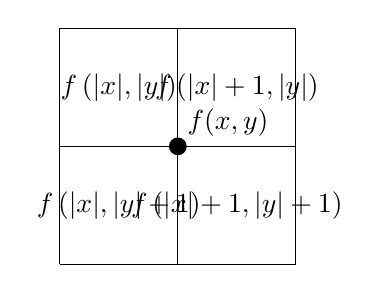
\begin{tikzpicture}[scale=1.5]
    \draw (0,0) grid (2,2);
    \node at (0.5,1.5) {$f\left(|x|,|y|\right)$};
    \node at (1.5,1.5) {$f\left(|x|+1,|y|\right)$};
    \node at (0.5,0.5) {$f\left(|x|,|y|+1\right)$};
    \node at (1.5,0.5) {$f\left(|x|+1,|y|+1\right)$};
    \filldraw (1,1) circle (2pt) node[above right] {$f(x,y)$};
\end{tikzpicture}
\caption{双线性插值}
\end{figure}

\begin{equation}
f(i+u,j+v) = (1-u)(1-v)f(i,j) + u(1-v)f(i+1,j) + (1-u)vf(i,j+1) + uvf(i+1,j+1)
\tag{5.3.10}
\end{equation}

式中,$x = i+u$,$y = j+v$,$i$ 和 $j$ 是 $x$ 和 $y$ 的整数部分,$u$ 和 $v$ 是 $x$ 和 $y$ 的小数部分。

### 5.3.2 模型建立

针对同时存在平移、选择和尺度变化的视频,假设相似变换模型

\begin{equation}
\begin{bmatrix}
x_i \\
y_i
\end{bmatrix}
= s
\begin{bmatrix}
\cos\theta & \sin\theta \\
-\sin\theta & \cos\theta
\end{bmatrix}
\begin{bmatrix}
x_i \\
y_i
\end{bmatrix}
+
\begin{bmatrix}
\Delta x \\
\Delta y
\end{bmatrix}
\tag{5.3.11}
\end{equation}

为求解该模型,需要代入 2 个匹配点计算运动参数。采用 SIFT 算法进行特征点识别,建立特征点集(详见 5.5.1)利用特征点集估计出抖动带来的变焦系数,代入相似变换模型,通过最小二乘法估计平移和旋转参数。

假设当前帧和参考帧分别为 \( f_i \) 和 \( f_j \),使用当前帧和参考帧的特征点集与特征集中心位置的变化率估计变焦系数 \( s \),建模过程如下:

当前帧图像 \( f_i \) 中的特征点集中心坐标:
\[
\begin{cases}
\overline{x}_i = \frac{1}{N} \sum_{k=1}^N x_{ik} \\
\overline{y}_i = \frac{1}{N} \sum_{k=1}^N x_{ik}
\end{cases}
\tag{5.3.12}
\]

式中,\( k=1, 2, \ldots, N \),则当前帧 \( f_i \) 和 \( f_j \) 中的特征点到点集中心的欧氏距离写为:
\[
d_k = \sqrt{(x_{ik} - \overline{x}_i)^2 + (y_{ik} - \overline{y}_i)^2}
\tag{5.3.13}
\]
\[
d_k = \sqrt{(x_{jk} - \overline{x}_j)^2 + (y_{jk} - \overline{y}_j)^2}
\tag{5.3.14}
\]

式中,\( k=1, 2, \ldots, N \),则 \( f_i \) 和 \( f_j \) 的变焦系数为
\[
s = \frac{\sum_{k=1}^N d_k * d_k'}{\sum_{k=1}^N d_j * d_j'}
\tag{5.3.15}
\]

直接求解相似变换模型,将所求是 \( N \) 对匹配特征点代入方差,得到
\[
\begin{pmatrix}
x_{ik} \\
y_{ik}
\end{pmatrix}
=
\begin{pmatrix}
\cos \theta & -\sin \theta \\
\sin \theta & \cos \theta
\end{pmatrix}
\begin{pmatrix}
sx_{jk} \\
sy_{jk}
\end{pmatrix}
+
\begin{pmatrix}
\Delta x \\
\Delta y
\end{pmatrix}
\tag{5.3.16}
\]

式中,\( k=1, 2, \ldots N \),将 \( t \) 特征点代入方程可得
\[
\begin{cases}
x_{i1} = asx_{j1} - bsy_{j1} + \Delta x \\
y_{i1} = bsx_{j1} + asy_{j1} + \Delta y \\
x_{i2} = asx_{j2} - bsy_{j2} + \Delta x \\
y_{i2} = bsx_{j2} + asy_{j2} + \Delta y \\
\ldots \\
x_{iN} = asx_{jN} - bsy_{jN} + \Delta x \\
y_{iN} = bsx_{jN} + asy_{jN} + \Delta y
\end{cases}
\tag{5.3.17}
\]

令
\[
\mathbf{B} = \begin{bmatrix}
x_{i1} \\
y_{i1} \\
\vdots \\
x_{iN} \\
y_{iN}
\end{bmatrix}, \quad
\mathbf{A} = \begin{bmatrix}
sx_{j1} & -sy_{j1} & 1 & 0 \\
sy_{j1} & sx_{j1} & 0 & 1 \\
\vdots & \vdots & \vdots & \vdots \\
sx_{jN} & -sy_{jN} & 1 & 0 \\
sy_{jN} & sx_{jN} & 0 & 1
\end{bmatrix}, \quad
\mathbf{X} = \begin{bmatrix}
a \\
b \\
\Delta x \\
\Delta y
\end{bmatrix}
\]

则方程组可以表示
\begin{equation}
\mathbf{B} = \mathbf{A} \mathbf{X}
\tag{5.3.18}
\end{equation}

对上述方差,解线性最小二乘方程组,其解为
\begin{equation}
\mathbf{X} = (\mathbf{A}^{\mathrm{T}} \mathbf{A})^{-1} \mathbf{A}^{\mathrm{T}} \mathbf{B}
\tag{5.3.19}
\end{equation}

在相似变换模型中,同时存在平移和旋转运动,平移由摄像机主动扫描形成,旋转由摄像机倾斜抖动造成。

对于存在主动扫描的平移运动,我们对其进行动态建模,考虑水平方向的平移运动,假设其速度变化量为 \(\Delta v\),在状态模型中 \(\Delta v\) 服从高斯分布,则状态模型为:
\begin{equation}
\begin{bmatrix}
\Delta x \\
\Delta v_x
\end{bmatrix}^{k+1} =
\begin{bmatrix}
1 & 1 \\
0 & 1
\end{bmatrix}
\begin{bmatrix}
\Delta x \\
\Delta v_x
\end{bmatrix}^k +
\begin{bmatrix}
0 \\
N(0, \sigma_x)
\end{bmatrix}
\tag{5.3.20}
\end{equation}
式中,\(\Delta v_x\) 为 \(\Delta x\) 的变化量,\(N(0, \sigma_x)\) 为高斯白噪声。

用参数 \(\theta\) 表示摄像头的倾斜,可以将其认为是一个随机序列,所以相应的状态模型为
\begin{equation}
\theta^{k+1} = \theta^k + N(0, \sigma_\theta)
\tag{5.3.21}
\end{equation}

得到相似变换模型的完整状态方程如下:
\begin{equation}
\begin{bmatrix}
\theta \\
\Delta x \\
\Delta v_x \\
\Delta y \\
\Delta v_y
\end{bmatrix}^{k+1} =
\begin{bmatrix}
1 & 0 & 0 & 0 & 0 \\
0 & 1 & 1 & 0 & 0 \\
0 & 0 & 1 & 0 & 0 \\
0 & 0 & 0 & 1 & 1 \\
0 & 0 & 0 & 0 & 1
\end{bmatrix}
\begin{bmatrix}
\theta \\
\Delta x \\
\Delta v_x \\
\Delta y \\
\Delta v_y
\end{bmatrix}^k +
\begin{bmatrix}
N(0, \sigma_\theta) \\
0 \\
N(0, \sigma_x) \\
0 \\
N(0, \sigma_y)
\end{bmatrix}
\tag{5.3.22}
\end{equation}
式中,\(\sigma_\theta\),\(\sigma_x\),\(\sigma_y\) 等参数相互独立

把计算得到的 \((\theta, \Delta x, \Delta y)\) 作为观测值,得到观测方程

\begin{equation}
\begin{bmatrix}
\theta \\
\Delta x \\
\Delta y
\end{bmatrix}^{k+1} =
\begin{bmatrix}
\theta \\
\Delta x \\
\Delta y
\end{bmatrix} +
\begin{bmatrix}
N(0, \sigma_{\theta}) \\
N(0, \sigma_{x}) \\
N(0, \sigma_{y})
\end{bmatrix}
\tag{5.3.23}
\end{equation}

由此建立了状态方程和观测方程,其中 $(\theta, \Delta x, \Delta y)$ 是相似变换模型中当前帧相对于参考帧的全局运动矢量参数变化。用 kalman 滤波公式对全局运动矢量参数 $(\theta, \Delta x, \Delta y)$ 进行平滑滤波。假设参考帧的位置为零,则全局运动矢量为绝对位移矢量,用全局运动矢量与 kalman 滤波得到的主动扫描运动分量相减得到抖动分量,将补偿参数代入相似变换模型,即可获得补偿后图像像素值。

\begin{table}[h]
\centering
\caption{表 5.3.1 视频稳像算法步骤}
\begin{tabular}{l}
\hline
\textbf{算法 5:运动路径估计和图像补偿} \\
\hline
输入:视频序列 X.mat 文件 \\
1. 对数据矩阵每个列向量建立动态模型和观测模型; \\
2. 用 kalman 滤波对式 (5.3.21) 计算结果进行平滑滤波,计算补偿参数; \\
3. 补偿参数代入式 (5.3.20) 进行插值补偿。 \\
\hline
\end{tabular}
\end{table}

\subsection{5.3.3 模型求解与结果分析}

在 Matlab2016a 的编译环境下编译算法,对附件 2 中带抖动的 4 组视频进行了稳像处理,在将经稳像处理后的视频用 Vibe 法进行前景目标提取,运行结果如表 5.3.2 所示。

从表 5.3.2 中可以看出,在进行视频稳像前 Vibe 算法对视频的前景识别出现了大量的重影,并且背景中物体的轮廓比较明显,包括树木、建筑物、道路护栏。从稳像处理后的图像来看,用本文算法处理后,有效地去除了视频抖动,但图像 car6 依然有背景噪点,图像 people1 和 people2 前景目标内也出现了空洞,这可能是因为 kalman 滤波仅是对抖动分量进行平滑处理,并没有完全去除抖动造成的。

如图 5.3.2 所示,由 kalman 滤波得到的噪声部分进行的平滑处理,即表示视频的抖动分量,从图像中我们可以看出视频拍摄时的抖动分量在经过平滑处理后曲线比起表示噪声的随机值曲线变得更加趋于平缓。

\begin{table}
\centering
\caption{视频稳像结果提取}
\begin{tabular}{c c c c}
\multirow{3}{*}{测试图} & \includegraphics[width=0.2\textwidth]{image1} & \includegraphics[width=0.2\textwidth]{image2} & \includegraphics[width=0.2\textwidth]{image3} \\
 & \includegraphics[width=0.2\textwidth]{image4} & \includegraphics[width=0.2\textwidth]{image5} & \includegraphics[width=0.2\textwidth]{image6} \\
 & \includegraphics[width=0.2\textwidth]{image7} & \includegraphics[width=0.2\textwidth]{image8} & \includegraphics[width=0.2\textwidth]{image9} \\
\multirow{3}{*}{基准图} & \includegraphics[width=0.2\textwidth]{image10} & \includegraphics[width=0.2\textwidth]{image11} & \includegraphics[width=0.2\textwidth]{image12} \\
 & \includegraphics[width=0.2\textwidth]{image13} & \includegraphics[width=0.2\textwidth]{image14} & \includegraphics[width=0.2\textwidth]{image15} \\
 & \includegraphics[width=0.2\textwidth]{image16} & \includegraphics[width=0.2\textwidth]{image17} & \includegraphics[width=0.2\textwidth]{image18} \\
\multirow{3}{*}{未做稳像处理} & \includegraphics[width=0.2\textwidth]{image19} & \includegraphics[width=0.2\textwidth]{image20} & \includegraphics[width=0.2\textwidth]{image21} \\
 & \includegraphics[width=0.2\textwidth]{image22} & \includegraphics[width=0.2\textwidth]{image23} & \includegraphics[width=0.2\textwidth]{image24} \\
 & \includegraphics[width=0.2\textwidth]{image25} & \includegraphics[width=0.2\textwidth]{image26} & \includegraphics[width=0.2\textwidth]{image27} \\
\multirow{3}{*}{稳像处理} & \includegraphics[width=0.2\textwidth]{image28} & \includegraphics[width=0.2\textwidth]{image29} & \includegraphics[width=0.2\textwidth]{image30} \\
 & \includegraphics[width=0.2\textwidth]{image31} & \includegraphics[width=0.2\textwidth]{image32} & \includegraphics[width=0.2\textwidth]{image33} \\
 & \includegraphics[width=0.2\textwidth]{image34} & \includegraphics[width=0.2\textwidth]{image35} & \includegraphics[width=0.2\textwidth]{image36} \\
\end{tabular}
\begin{tabular}{c c c c}
(a) cars6 & (b) cars7 & (c) people1 & (d) people2 \\
第30帧 & 第24帧 & 第40帧 & 第30帧 \\
\end{tabular}
\end{table}

\section{问题四模型的建立及求解}

\subsection{问题模型建立}

本问题的本质是在前述背景建模方法的基础上对提取前景目标二值图进行判别并输出视频帧号。其模型方法流程图 5.4.1。

根据前面对视频类型的分类:静态背景、动态背景和相机抖动,可以将附件 3 中提供的 8 组视频进行分类,并选择合适的模型算法进行前景目标提取。通过视频类型判断,可将这 8 组视频分类如表 5.4.1。

根据各类前述背景建模方案的适用性,本文决定对静态背景视频采用 MOG 法进行前景提取识别,对动态背景视频采用改进的 VIBE 法进行前景提取识别。为了能够自动地提取相应视频包含显著前景目标视频帧标号,本文在 Matlab 编码中嵌入帧标号记录模块,当在视频中提取到前景目标时,算法能够自动记录视频帧标并统一输出。

\begin{figure}[h]
    \centering
    \begin{subfigure}[t]{0.45\textwidth}
        \centering
        \includegraphics[width=\textwidth]{image_a.png}
        \caption{(a) cars6}
    \end{subfigure}
    \hfill
    \begin{subfigure}[t]{0.45\textwidth}
        \centering
        \includegraphics[width=\textwidth]{image_b.png}
        \caption{(b) cars7}
    \end{subfigure}
    
    \begin{subfigure}[t]{0.45\textwidth}
        \centering
        \includegraphics[width=\textwidth]{image_c.png}
        \caption{(c) people1}
    \end{subfigure}
    \hfill
    \begin{subfigure}[t]{0.45\textwidth}
        \centering
        \includegraphics[width=\textwidth]{image_d.png}
        \caption{(d) people2}
    \end{subfigure}
    \caption{时间序列帧数-垂直方向位移矢量关系图}
    \label{fig:5.3.2}
\end{figure}

\begin{figure}[h]
    \centering
    \includegraphics[width=0.8\textwidth]{image_flowchart.png}
    \caption{提取包含显著前景目标视频帧标号流程图}
    \label{fig:5.4.1}
\end{figure}

\begin{table}[h]
\centering
\begin{tabular}{c c c c c c c c}
\hline
 & hall & & Lobby & & office & & overpass \\
\hline
1 & 单帧 & 连帧 & 单帧 & 连帧 & 单帧 & 连帧 & 单帧 \\
 & & & & & & & 连帧 \\
\hline
2 & 795 & 1-512 & 79 & 154-198 & 197 & 583-1137 & 374 \\
 & & & & & & & 547-679 \\
\hline
3 & 1138 & 599-739 & 259 & 345-1038 & 372 & 1265-1324 & 968 \\
 & & & & & & & 2335-2962 \\
\hline
4 & 1246 & 819-1054 & 521 & 622-668 & 501 & 1415-1508 & 1551 \\
 & & & & & & & \\
\hline
5 & & 1153-1213 & 870 & 963-1038 & 2080 & 1642-1793 & 1881 \\
 & & & & & & & \\
\hline
6 & & 1278-1543 & 1161 & 1239-1283 & & 1826-2043 & 2098 \\
 & & & & & & & \\
\hline
7 & & 1556-2583 & & 1334-1538 & & & \\
 & & & & & & & \\
\hline
8 & & 2721-2779 & & & & & \\
 & & & & & & & \\
\hline
9 & & 2816-2869 & & & & & \\
 & & & & & & & \\
\hline
10 & & 2904-2921 & & & & & \\
 & & & & & & & \\
\hline
11 & & 3025-3347 & & & & & \\
 & & & & & & & \\
\hline
12 & & 3415-3534 & & & & & \\
 & & & & & & & \\
\hline
\end{tabular}
\caption{包含显著前景目标视频帧标号(静态背景视频)}
\end{table}

\begin{table}[h]
\centering
\begin{tabular}{c c c c c c c c}
\hline
 & Campus & & Curtain & & Escalator & & Fountain \\
\hline
1 & 单帧 & 连帧 & 单帧 & 连帧 & 单帧 & 连帧 & 单帧 \\
 & & & & & & & 连帧 \\
\hline
2 & 85 & 200-225 & 411 & 1760-1903 & 2415 & 1-154 & 141 \\
 & & & & & & & 157-211 \\
\hline
3 & 600 & 306-523 & 967 & 2173-2314 & 2539 & 236-2394 & 259 \\
 & & & & & & & 408-523 \\
\hline
4 & 1193 & 637-683 & 1561 & 2768-2931 & 2754 & 2773-3417 & 335 \\
 & & & & & & & \\
\hline
5 & 1264 & 687-712 & 2126 & & & & \\
 & & & & & & & \\
\hline
6 & & 737-904 & 2642 & & & & \\
 & & & & & & & \\
\hline
7 & & 1003-1037 & & & & & \\
 & & & & & & & \\
\hline
8 & & 1329-1374 & & & & & \\
 & & & & & & & \\
\hline
9 & & 1378-1407 & & & & & \\
 & & & & & & & \\
\hline
\end{tabular}
\caption{包含显著前景目标视频帧标号(动态背景视频)}
\end{table}

\subsection{5.5 问题五模型的建立及求解}

\subsubsection{5.5.1 匹配特征点的生成}

\subsubsection*{(一) SIFT 特征点检测}

SIFT 算法\cite{12-13}首先对图像进行高斯差分金字塔得到高斯差分图像,对得到的高斯差分图像在多尺度范围内进行关键点检测,对检测到的关键点,使用高斯模板在邻域范围得到关键点的梯度直方图,根据局部图像的梯度方向,对每一个关键点指定一个或多个方向。

为了清晰地说明这个问题,我们将 SIFT 算法分解为表 5.5.1 中的四步:

\begin{table}[h]
\centering
\caption{SIFT 算法步骤}
\begin{tabular}{|p{16cm}|}
\hline
算法 6: SIFT 算法: \\
\hline
1. 尺度空间极值检测:搜索所有尺度上的图像位置。通过高斯微分函数来识别潜在的对于尺度和旋转不变的兴趣点; \\
2. 关键点定位:在每个候选的位置上,通过一个拟合精细的三维二次函数来确定位置和尺度。关键点的选择依据于它们的稳定程度; \\
3. 方向确定:基于图像局部的梯度方向,分配给每个关键点位置一个或多个方向。所有后面的对图像数据的操作都相对于关键点的方向、尺度和位置进行变换,从而提供对于这些变换的不变性; \\
4. 关键点描述:在每个关键点周围的邻域内,在选定的尺度上测量图像局部的梯度。这些梯度被变换为一种表示,这种表示允许比较大的局部形状的变形和光照变化。 \\
\hline
\end{tabular}
\end{table}

\subsubsection*{(1) 尺度空间极值检测}

关键点检测的第一步是能重复地对同一个物体从不同视角,确定关键点的位置和尺度。这可以通过使用连续的尺度函数来实现。

令 $L(x, y, \sigma)$ 为图像的尺度空间,其定义如下:

\begin{equation}
L(x, y, \sigma) = G(x, y, \sigma) * I(x, y)
\tag{5.5.1}
\end{equation}

其中 $G(x, y, \sigma)$ 是高斯函数,$G(x, y, \sigma) = \frac{1}{2\pi\sigma^2}e^{-(x^2 + y^2)/2\sigma^2}$,$\sigma$ 是尺度因子。

设高斯金字塔共 $o$ 组、$S$ 层,则第 $s$ 层的尺度为

组内相邻层尺度化简为
\begin{equation}
\sigma(s) = \sigma_0 \cdot 2^{s/S}
\tag{5.5.2}
\end{equation}

相邻组的尺度可化为
\begin{equation}
\sigma_{s+1} = \sigma_s \cdot 2^{1/S}
\tag{5.5.3}
\end{equation}

则组内各层的尺度为
\begin{equation}
\sigma_{o+1}(s) = \sigma_o \cdot 2^{s+S/S} = 2\sigma_o \cdot 2^{s/S}
\tag{5.5.4}
\end{equation}
\begin{equation}
2^{i-1}(\sigma, k\sigma, k^2\sigma, \dots k^{n-1}\sigma)
\tag{5.5.5}
\end{equation}

其中,$k = 2^{1/S}$,$i$ 为金字塔组数,$n$ 为每一组层数。

如图 5.5.1 所示,我们选用了高斯差分金字塔,首先因为高斯差分函数的计算效率比较高,高斯差分算子可以简单的通过高斯模糊图像相减来得到,其次高斯差分函数提供了一个近似尺度标准化的高斯拉普拉斯算子的近似。DoG 算子与图像的卷积的定义如下:
\begin{equation}
\begin{aligned}
D(x, y, \sigma) &= \big(G(x, y, k\sigma) - G(x, y, \sigma)\big)G(x, y, \sigma) \\
&= L(x, y, k\sigma) - L(x, y, \sigma)
\end{aligned}
\tag{5.5.6}
\end{equation}

在这里,我们将第 0 层的初始尺度定为 1.6,图像的初始尺度为 0.5,故第 0 层的实际尺度为
\begin{equation}
\sqrt{1.6 \times 1.6 - 0.5 \times 0.5} = 1.52
\tag{5.5.7}
\end{equation}

首先对原始图像升采样,来构建层,则扩展一倍构建的层的尺度为:
\begin{equation}
\sqrt{1.6 \times 1.6 - (2 \times 0.5) \times (2 \times 0.5)} = 1.25
\tag{5.5.8}
\end{equation}

\begin{figure}[h]
\centering
\includegraphics[width=0.8\textwidth]{image.png}
\caption{高斯差分金字塔}
\label{fig:5.5.1}
\end{figure}

(2) 关键点定位

通过将一个像素与周围像素比较得到了待定的关键点后,还需要一个精确的确定关键点的位置、尺度和主曲率的比值。通过精确定位和主曲率的值,就可以精确定位极值点,同时去除边缘点。

利用 DoG 函数在尺度空间的泰勒展开式

\begin{equation}
D(x) = D + \frac{\partial D^T}{\partial x} x + \frac{1}{2} x^T \frac{\partial^2 D}{\partial x^2} x
\tag{5.5.9}
\end{equation}

求导并令方程的值为零,得到极值点的修正偏移量为

\begin{equation}
\hat{x} = -\frac{\partial^2 D^{-1}}{\partial x^2} \frac{\partial D}{\partial x}
\tag{5.5.10}
\end{equation}

对应极值点,得到方程的值为

\begin{equation}
\hat{D} = D + \frac{1}{2} \frac{\partial D^T}{\partial x} \hat{x}
\tag{5.5.11}
\end{equation}

借助于 Lowe\(^{[14]}\) 的研究,在这里我们将 \(D(x)\) 大于 0.03 的值保留,否则删除。

(3) 方向确定

通过根据图像的局部性质,对每个关键点指定一致的方向,关键点描述子用这个方向来表示。像素点的梯度表示为

\begin{equation}
grad(x, y) = \left( \frac{\partial I}{\partial x}, \frac{\partial I}{\partial y} \right)
\tag{5.5.12}
\end{equation}

对每一个图像样本 \(L(x, y)\),梯度的模值和方向计算如下

\begin{equation}
m(x, y) = \sqrt{\left( L(x+1, y) - L(x-1, y) \right)^2 + \left( L(x, y+1) - L(x, y-1) \right)^2}
\tag{5.5.13}
\end{equation}

\begin{equation}
\theta(x, y) = \tan^{-1} \left[ \frac{L(x, y+1) - L(x, y-1)}{L(x+1, y) - L(x-1, y)} \right]
\tag{5.5.14}
\end{equation}

方向直方图是由关键点周围样本点的梯度方向来组成的,方向直中每个柱的变化范围为 10 度。方向直方图中最大的位置即设置为该关键点的主方向。

(4) 关键点描述

1. 从高斯差分图像中得到关键点的邻域范围,对该邻域范围内的样本点进行直方图运算,邻域半径的计算公式为

\begin{equation}
radius = \frac{3\sigma_{oct} \times \sqrt{2} \times (d+1) + 1}{2}
\tag{5.5.15}
\end{equation}

其中,$d$ 是样本点到直方图块间隔中心点的距离,$\sigma_{oct}$ 为差分空间的尺度。

2. 由得到的关键点的主方向对坐标轴旋转,变换矩阵为
\begin{equation}
\begin{pmatrix}
\bar{x} \\
\bar{y}
\end{pmatrix}
=
\begin{pmatrix}
\cos\theta & -\sin\theta \\
\sin\theta & \cos\theta
\end{pmatrix}
\begin{pmatrix}
x \\
y
\end{pmatrix}
\tag{5.5.16}
\end{equation}

3. 对关键点周围 $16 \times 16$ 个样本点的梯度幅度乘以权重系数,生成方向直方图,其中,权重系数为
\begin{equation}
weight = |grad(I_{\sigma}(x, y))| \times \exp\left(-\frac{x_k^2 + y_k^2}{2\sigma_w^2}\right) \times (1-d_r) \times (1-d_c) \times (1-d_o)
\tag{5.5.17}
\end{equation}

(二)SIFT 关键点匹配

本文分别对当前帧和参考帧建立“关键点描述子”集合,使用欧氏距离分别对两个集合进行匹配,从而实现对检测到的关键点进行匹配。

穷举匹配法匹配示意图如图 5.5.2 所示:

\begin{figure}[h]
\centering
\includegraphics[width=0.8\textwidth]{image.png} % 替换为实际图片路径
\caption{穷举匹配}
\label{fig:exhaustive_matching}
\end{figure}

我们采用 Best-Bin-First (BBF) 法进行特征匹配,论文中我们只考虑了最近邻域和次近邻域比值小于 0.8 的匹配点。

\subsection{5.5.2 单应矩阵与 FOV 线的生成}

单应矩阵 $H = \left(h_{ij}\right)_{3 \times 3}$,取 $h_{3 \times 3} = 1$

由两平面间的射影变换可建立如下方程:
\begin{equation}
\begin{bmatrix}
x_1 & y_1 & 1 & 0 & 0 & 1 & -u_1x_1 & -u_1y_1 \\
0 & 0 & 0 & x_1 & y_1 & 1 & -v_1x_1 & -v_1y_1
\end{bmatrix}
h =
\begin{bmatrix}
u_1 \\
v_1
\end{bmatrix}
\tag{5.5.18}
\end{equation}

式中,$h = (h_{11}, h_{12}, h_{13}, h_{21}, h_{22}, h_{23}, h_{31}, h_{32}, h_{33})^T$。利用 5.5.1 中计算的关键点,采用奇异值分解(SVD)的最小二乘法计算矩阵 H。由单应矩阵得到图像在另一视角下的透射变换图像,根据图像边界点计算生成摄像机的摄像机视野 FOV (FOV: field of view) 分界线。

\subsection*{5.5.3 目标匹配}

在目标匹配时,采用以下算法:

\begin{table}[h]
\centering
\caption{目标匹配算法}
\begin{tabular}{|p{16cm}|}
\hline
算法 7:目标匹配算法 \\
输入:数据矩阵 X,子空间个数 n \\
1. 利用 5.2 中改进 VIBE 算法在摄像机 1、2 中分别检测目标,利用式 5.5.11 中的算法统计两摄像机在公共 FOV 中的目标数量,如果目标数量相等,进入下一步; \\
2. 利用式 5.5.16 提取需要交接的目标位置 $P_i^k (i=1,2,3\cdots,N; k=1,2)$,其中 N 表示摄像机公共 FOV 区域中目标数量,$P_i^k$ 表示第 k 个摄像机公共 FOV 区域中的第 i 个目标; \\
3. 利用单应矩阵计算摄像机 1 中的目标的透射变换位置 $\overline{P}_i^1$,计算 $\overline{P}_i^1 \overline{P}_j^2$ 的距离 $\|\overline{P}_i^1 \overline{P}_j^2\| (i,j=1,2,3\cdots N)$; \\
4. 对 $\|\overline{P}_i^1 \overline{P}_j^2\|$ 升序排序,选择前 N 个最小值,则 $P_i^1$、$P_j^2$ 位置处的目标即为匹配的目标。 \\
\hline
\end{tabular}
\end{table}

\subsection*{5.5.4 模型求解与分析}

\subsubsection{(一) SIFT 特征点求解与分析}

\begin{figure}[h]
    \centering
    \includegraphics[width=\textwidth]{image1.png}
    \caption{(a)}
\end{figure}

\begin{figure}[h]
    \centering
    \includegraphics[width=\textwidth]{image2.png}
    \caption{(b)}
\end{figure}

\begin{figure}[h]
    \centering
    \includegraphics[width=\textwidth]{image3.png}
    \caption{(c)}
\end{figure}

\begin{figure}[h]
    \centering
    \includegraphics[width=\textwidth]{image4.png}
    \caption{(d)}
\end{figure}

\begin{figure}[h]
    \centering
    \caption{图 5.5.3 特征点识别匹配提取图}
\end{figure}

试验得出算法识别提取的匹配特征点数目与两帧图片的相似度呈正相关。图 5.5.3(d) 为同一视角下不同时刻的截图,图像背景具有极大的相似性;因此,其匹配点和特征点数目显著高于其他图像。图 5.5.3(a) 中,识别到 1033 个特征点,其中匹配的只有 8 个;这是因为进行关键点定位后,算法将许多 $D(x)$ 大于 0.3 的点、对比度的关键点和不稳定的边缘响应点抛弃了,增强了匹配稳定性。

\section*{(二) 目标匹配结果与分析}

\begin{figure}[h]
    \centering
    \includegraphics[width=\textwidth]{image1.png}
    \caption{SIFT 特征点匹配}
    \label{fig:5.5.4}
\end{figure}

\begin{figure}[h]
    \centering
    \includegraphics[width=\textwidth]{image2.png}
    \caption{目标交接检测结果}
    \label{fig:5.5.5}
\end{figure}

一般而言,选择的 SIFT 匹配点越多、分布范围越广,计算的 FOV 分界线越稳定和准确,因此后续的目标交接也会越准确。本文中计算出的匹配数量为 7 时,此时未能实现目标检测;通过人工干预增加 3 个匹配点后,实现了目标的检车。基于这一思想,我们认为人工干预增加匹配点的方式,为解决有遮挡以及匹配点非共面这类情况下重叠视域运动目标的检测提供了一种研究方向。

\section*{5.6 问题六模型的建立及求解方案}

\subsection{5.6.1 问题背景及解析}

\subsubsection{(一) 问题背景}

近来,恐怖袭击和突发性群体事件不断挑战城市的防御底线,公共安全问题已在全球范围内引起广泛关注。传统的视频监控主要依赖于人工监控,费时费力且效率低,智能视频监控系统的实现成为了减少公共场合内群众人身伤害及财产损失的有效措施。因此,对基于视频监控的群体异常行为检测系统进行深入研究具有重要的应用价值与现实意义。群体异常事件检测旨在从视频序列中挖掘出隐藏着的、潜在的有用的信息,并结合合适的模式识别模型,将正常行为和异常行为区分开来。其中所进行的群体行为分析,其实质就是从图像序列中提取出有效的特征,然后对这些特征进行分析从而确定出该行为所属类别。

在群体异常检测领域中,群体异常事件检测方法大致分为三大类。第一类是以传统的基于目标的方法,该类方法将群体仍然考虑成由单个目标所组成。因此,

群体行为的理解就又转换到了传统的单个目标的分析的过程,比如目标检测、分割及跟踪。但是,这种方法也忽略了人与人之间的相互作用性,同时计算速度也会受到目标数量的影响。第二类是从整个监控场景出发来分析,提取场景中特别的信息特征。一种经典的方法是利用光流来刻画场景的运动特征。不幸的是,光流除了运算速度上的缺点之外,还易受光照的影响。第三类是将前两种方式结合起来,既分析整个监控场景又跟踪某些单个目标。但是,这种方法有很大的运算负荷,计算效率低下。目前,第二类方法得到了很大程度的认同,并得到了广泛的研究。

\section*{(二) 群体异常行为事件特征分析}

本节主要研究人群惊慌逃散这个异常行为事件,详细分析了人群惊慌逃散事件的特点,并对这些内容简述如下:

人群惊慌逃散事件不同于一般的群体事件,它具有非常显著的特点:1、人群密度较大;2、运动较剧烈;3、运动方向杂乱无章。因此,可以利用这些区别,从视频序列图像中提取相对应的密度特征和运动特征,用来区分人群惊慌逃散事件和正常的群体事件。经过分析对比,在实验中,我们主要考虑以下几类特征:

(1)人群密集成度:人群密集成度可以反映人群的规模即图像中大概的人数是多还是少,人群密集成度达到一定程度才能判断为群体事件。我们为了定量的衡量行人分布集中程度的大小,引入了信息论中熵的概念。在信息论中,熵是随机变量不确定度的度量。如果把场景中行人的分布情况看作为一个随机事件,也就是把包含行人分布情况信息的前景图像的分布作为一个离散型随机变量看待。前景图像在 \(x\) 轴和 \(y\) 轴上各处的分布概率可以直接从前景图像积分投影估计中得到。

(2)运动强度均值:运动强度均值反映了视频序列图像中运动对象的平均运动强度,该值越大,表示发生人群惊慌逃散事件的可能性也就越大。该指标可以人群运动的平均速度来加以评价。

(3)运动方向直方图的方差:虽然运动强度均值能够从整体上描述人群惊慌逃散事件,但是在大多数情况下,比如游行或多人行走等正常群体事件中的运动强度均值可能和人群惊慌逃散事件的运动强度均值相差不大,那么仅仅用这一个运动特征很难将这两类事件区分开来。因此,需要一个能够描述运动方向分布

的特征来和运动强度均值结合起来检测。所以,引入了运动方向直方图的方差这个特征,它能够反映运动方向的分布情况。

(4) 为了和后面的聚集事件区分开来,我们还引入了另一个群体事件的特征进行分析,就是运动像素数。运动像素数与前景像素数不同,它是用来描述前景像素中运动的一部分像素的多少。

\subsection*{5.6.2 模型建立}

(一) 数学模型

\begin{equation}
I =
\begin{cases}
1 & \text{yes} \quad T_i \geq T_j \\
0 & \text{no} \quad \text{else}
\end{cases}
\tag{5.6.1}
\end{equation}

式中,$T_i$ 为各检测指标计算值,$T_j$ 为各检测指标阈值。

该算法通过指标判别模型,对分布熵、角点运动速度、运动方向直方图方差 $\sigma_{\text{angle}}$、运动像素数 $N_{\text{um\_mp}}$ 等指标进行检测,进而判断视频中是否出现人群异常行为。

(二) 模型建立过程

模型建立流程如图 5.6.1 所示

Step.1 运动目标提取:通过问题 2 中的改进 VIBE 模型对监控场景进行建模,然后运用背景差法,得到运动前景图像。

Step.2 前景图像的空间分布(人群分布):为了表示人群在空间的分布情况,首先将每一帧的前景图像分别投影到图像坐标系(图像坐标系原点为图像的左下角)的 $x$ 轴和 $y$ 轴,建立前景图像在垂直和水平方向的积分投影直方图,用 $\mathbf{h}_x(i)$ 和 $\mathbf{h}_y(j)$ 分别表示为

\begin{equation}
\mathbf{h}_x(i) = \{k_i, 0 \leq i < W\}
\tag{5.6.2}
\end{equation}

\begin{equation}
\mathbf{h}_y(j) = \{q_j, 0 \leq j < H\}
\tag{5.6.3}
\end{equation}

式中,$k_i$ 和 $q_j$ 分别代表前景像素在 $x$ 轴上 $i$ 处和 $y$ 轴上 $j$ 处的投影数量;$W$ 和 $H$ 代表图像的宽和高。

\begin{figure}[h]
    \centering
    \includegraphics[width=\textwidth]{image.png}
    \caption{模型建立及求解流程}
    \label{fig:flowchart}
\end{figure}

前景图像的积分投影直方图从直观上反映出了场景中行人在水平和垂直方向的集中程度。在这里,我们为了定量的衡量行人分布集中程度的大小,引入了信息论中熵(entropy)的概念,把场景中行人的分布情况看作为一个随机事件。参考熵在信息论中的定义,根据前景像素的概率分布,定义 x 轴和 y 轴两个方向上的分布熵 $H(x), H(y)$ 分别为

\begin{equation}
H(x) = \sum_{i=1}^{W} p_x(i) \log \frac{1}{p_x(i)}, p_x(i) \neq 0
\tag{5.6.4}
\end{equation}

\begin{equation}
H(y) = \sum_{j=1}^{H} p_y(i) \log \frac{1}{p_y(i)}, p_y(i) \neq 0
\tag{5.6.5}
\end{equation}

综合考虑场景中人群在水平和垂直方向上分布熵的大小,可以检测人群聚集

的发生为:
\begin{equation}
I = H(x) \times H(y)
\tag{5.6.6}
\end{equation}
为了便于检测和计算,对熵值进行归一化处理为:
\begin{equation}
I_{\max} = \log(W) \times \log(H)
\tag{5.6.7}
\end{equation}
\begin{equation}
I = 1 - \frac{H(x) \times H(y)}{I_{\max}}
\tag{5.6.8}
\end{equation}

Step.3 角点检测及光流跟踪:在本文中,选择 Harris 角点 \cite{15-16} 作为图像的特征点进行计算角点速度估计,用特征点的运动状态估计人群整体的运动状态;采用计算光流 \cite{17} 的方法来获取像素点的动态特征(位置、速度、方向、轨迹等)。角点运动速度 \( v \) 为:
\begin{equation}
v = \sqrt{d_x^2 + d_y^2} \times fps
\tag{5.6.9}
\end{equation}
式中,\( fps \) 为视频帧率,角点 \( \mathbf{u} \) 的速度矢量 \( d = \begin{bmatrix} d_x, d_y \end{bmatrix}^T \)。

在进行人群奔跑行为检测时,用特征点的平均运动速度来估计人群整体的运动速度,当人群整体平均运动速度超过预先设置的阈值时,认为人群发生剧烈的运动。

每一帧图像人群运动的平均速度 \( V_{avg} \) 定义为:
\begin{equation}
V_{avg} = \frac{1}{k} \times \sum_{i=1}^{k} v_i
\tag{5.6.8}
\end{equation}

Step.4 计算帧运动方向直方图的方差:首先利用 (3) 步中提到计算光流的算法提取出当前帧前景像素点的运动方向后,对运动方向进行量化为 0-7 共 8 个等级,统计对应方向的个数,计算帧内前景像素的平均方向 \( Angle_{avg} \):
\begin{equation}
Angle_{avg} = \frac{1}{8} \sum_{i=0}^{7} AngHist[i]
\tag{5.6.9}
\end{equation}
计算该帧运动方向直方图的方差 \( \sigma_{angle} \):
\begin{equation}
\sigma_{angle} = \sqrt{\frac{1}{8} \sum_{i=0}^{7} \left( AngHist[m] - Angle_{avg} \right)^2}
\tag{5.6.10}
\end{equation}

Step.5 运动像素数计算:利用 (3) 步中提到的计算光流的算法计算出当前帧

前景像素点的运动强度后,对运动强度大于阈值 \( V_0 \) 的像素点进行统计,得到运动像素数 \( N_{\text{um}_{\text{mp}}} \)。

\textbf{Step.6 异常事件识别} 利用这 4 个特征对视频进行处理,如果检测到异常群体事件,系统报警提醒。

\subsection{5.6.3 模型求解与分析}

考虑到人群惊慌逃散事件的特点,本文提出了一种基于整体特征的视频中人群异常行为检测算法;该算法通过指标判别模型,对分布熵、角点运动速度、运动方向直方图方差、运动像素数等指标进行检测,进而判断是否出现人群异常行为。

\subsubsection{(一) 前景目标检测及阴影消除}

在这里我们着重强调阴影去除的办法,因为在前景目标检测中,阴影和运动目标具有相似的运动特性,所以常常会把阴影区域错误地检测为前景区域,影响后续处理的结果。在实际的室外场景应用中,由于光照的存在,阴影常常会出现在图像中。因此,为了得到正确的结果,必须首先去除阴影。本文利用文献 \cite{ref18} 结合阴影的光学特征和纹理特征来检测阴影,处理结果对比如下:

\begin{figure}[h]
    \centering
    \includegraphics[width=\textwidth]{image1.png}
    \caption{原始图像}
\end{figure}

\begin{figure}[h]
    \centering
    \includegraphics[width=\textwidth]{image2.png}
    \caption{背景图像}
\end{figure}

\begin{figure}[h]
    \centering
    \includegraphics[width=\textwidth]{image3.png}
    \caption{运动目标图像}
\end{figure}

\begin{figure}[h]
    \centering
    \includegraphics[width=\textwidth]{image1.png}
    \caption{前景运动目标提取对比图}
    \label{fig:5.6.2}
\end{figure}

经实验分析发现,基于改进 VIBE 算法进行背景建模的背景差分法非常适用于光照条件变化较小的情况下的运动目标检测;该算法可提取到含有清晰轮廓的运动目标,且光影出现率低。此外,实验发现利用文献 [19-20] 的办法可以有效去除提取图像中的阴影。

\subsubsection{异常群体事件特征的阈值选取}

通过对不同数量行人在聚集过程中分布熵 $I$ 值直方图分析来估计人群聚集的阈值 $T_{1}$。

\begin{figure}[h]
    \centering
    \includegraphics[width=0.45\textwidth]{image2.png}
    \caption{10 人聚集视频}
    \label{fig:5.6.3}
\end{figure}
\begin{figure}[h]
    \centering
    \includegraphics[width=0.45\textwidth]{image3.png}
    \caption{15 人聚集视频}
    \label{fig:5.6.4}
\end{figure}

\begin{figure}[h]
    \centering
    \includegraphics[width=0.8\textwidth]{image1.png}
    \caption{20人聚集视频}
    \label{fig:20_people}
\end{figure}

对 10 人(人群聚集出现在 60 帧)、15 人(人群聚集出现在 63 帧)和 20 人(人群聚集出现在 33 帧)聚集情况下 $I$ 值的直方图分析发现,当 $I$ 值大于 0.3 时,人群聚集活动的发生,因此针对此类群体活动下将聚集阈值 $T_{1}$ 设为 0.3。

\begin{figure}[h]
    \centering
    \includegraphics[width=0.45\textwidth]{image2.png}
    \includegraphics[width=0.45\textwidth]{image3.png}
    \caption{前景运动目标集中图}
    \label{fig:foreground}
\end{figure}

这里我们应特别注意,当某一帧的 $I$ 值突然发生较大变化时,认为它是噪声,系统不发出报警信号。只有当连续 10 帧的 $I$ 值大于其阈值,认为发生了人群的聚集,系统报警。这个过程可以有效地减少误报警率。当场景中存在较少数量的行人时,如果行人间距离较近,其前景像素分布较为集中(如图 \ref{fig:foreground} 所示),从而导致分布熵 $I$ 值较高,这时会造成人群聚集的误报警。本文旨在检测与识别人群整体行为,当场景中行人数量较少时,对其进行聚集检测就没有意义。在设计中,根据前景像素数量与场景中的人数存在的线性关系,观察分析不同数量行人在该场景由远到近运动过程中其前景像素数量的变化。在进行行人的聚集检测时,以 10 人在场景中运动时,其前景像素数量的平均值在整帧图像中所占的比例 ($m/(W \times H) \geq 0.04$) 作为衡量是否为人群的依据,当行人在前景中所占像素达

到这一比例时,再进行人群聚集的检测,当低于这个比例时,将分布熵 I 的值设置为小于聚集阈值 \( T_1 \) 的一个常数。这样,就可以避免由于场景中行人较少而产生的人群聚集的误检测。

关于人群奔跑的阈值 \( T_2 \) 的设定,在设计中,我们通过对一定连续时间内场景中行人运动平均速度的分析估计人群奔跑的阈值 \( T_2 \),如图 5.6.7 所示。

\begin{figure}[h]
\centering
\includegraphics[width=\textwidth]{image.png}
\caption{视频帧平均速度 \( V_{avg} \)}
\end{figure}

通过对一定数量行人视频的统计分析发现。在同一固定场景下,人群中行人的正常平均运动速度曲线存在较小范围的波动,几乎成一条直线。在实验中,将人群的奔跑阈值 T2 设置为 40,当人群运动的平均速度 \( V_{avg} \) 持续大于 40 时,则可以认为发生了人群的奔跑行为。

用特征点的运动状态估计人群整体的运动状态,由于需要根据检测出的角点的运动估计行人的运动状态,而背景中固定的角点或者由于环境的干扰(风、光照等的影响)造成检测出的角点产生微小的移动,并不能够代表场景中行人的运动状态,因而需要从检测到的角点集合中删除背景中的固定角点和移动微小的角点,提取出运动的角点作为人群整体运动的特征。本次论文中,我们采用的删除非运动角点的方法是,首先获得含有待检测人群的连续 2 帧图像,即第 \( n \) 帧和第 \( (n+1) \) 帧,对第 \( n \) 帧图像进行 Harris 角点检测,将检测到的角点位置集合作为光流跟踪的初始点集合记为 \( P1 \);然后利用金字塔 L-K 光流算法 \({}^{[21]}\),对运动进行跟踪,在第 \( (n+1) \) 帧得到跟踪成功的角点位置集合,记为 \( P2 \)。对于 \( P1 \) 中的每

一个角点,判断其在 P2 中是否同样存在。若存在,则在 P2 中删除该角点,反之则将该角点保留在集合 P2 中,并对运动的角点进行标记。

为了避免由于人群运动速度正常波动造成的奔跑误报警,需要对的值进行峰值滤波处理。本文中我们采取的办法是,如果当前帧的 $V_{avg}$ 值为相邻连续 5 帧中的最小值或者最大值时,取这连续 5 帧的均值作为新的 $V_{avg}$ 的值。这样可以减小波动,同时不丢失原来的峰值特性。当 $V_{avg}$ 的值在某一帧突然发生较大的变化,认为其是噪声,系统不做出反应。只有当连续 5 帧 $V_{avg}$ 的值大于其阈值时,认为发生了人群的奔跑行为,系统发出报警信号。

\subsection*{5.6.4 模型评价}

优点:该方法不需要对单个行人进行分割以及样本的训练,可实现快速、准确地进行人群异常行为检测。在实验中,使用固定场景下拍摄的视频测试算法的性能,针对某一具体的固定场景,阈值经估计、设置完成后,本文方法能够保证在当前场景下准确、及时和有效地对人群聚集和奔跑行为进行检测和识别。另外,本文方法对硬件的要求较低,不需要高性能的监控设备,在较低分辨率下便能实时、有效地完成检测。

缺点:本文采用基于阈值的方法判断人群行为是否发生,阈值设置是否合理,直接影响检测与识别结果的有效性和准确性。本文只针对昼间正常光照条件下人群的聚集和奔跑行为的检测与识别进行了研究,没有考虑如何结合其他人群运动特征(如方向、轨迹等)在夜间或者光照不足等条件下实现对多种人群行为的检测与识别,忽略了人群信息的时空相关性。另外,对于一些和我们所定义的人群惊慌逃散事件、聚集事件具有相似特征的事件,例如足球场上的踢球事件,还需要设置其他合理的指标才能将这些事件很好的区分开来。

\section*{六、模型分析及展望}

\begin{table}
\centering
\caption{各类模型对比分析}
\begin{tabular}{|c|c|c|}
\hline
模型 & 优点 & 缺点 \\
\hline
帧差模型 & \begin{itemize}
    \item 实现简单;
    \item 程序设计复杂度低;
    \item 可适应动态环境变化。
\end{itemize} & \begin{itemize}
    \item 不利于低速移动的目标提取;
    \item 不能提取出对象的完整区域,只能提取出边界。
\end{itemize} \\
\hline
单高斯模型 (SGM) & \begin{itemize}
    \item 在固定背景下能够很好地去除噪点和背景;
    \item 适用于室内和场景单一的背景。
\end{itemize} & \begin{itemize}
    \item 运算量大,提取时间长;
    \item 不能完整识别前景轮廓,提取的前景目标出现空洞较多。
\end{itemize} \\
\hline
VIBE 模型 & \begin{itemize}
    \item 实现简单;
    \item 能快速、有效的提取前景目标;
    \item 程序设计复杂度低。
\end{itemize} & \begin{itemize}
    \item 存在鬼影(ghost)现象;
    \item 动态场景下将部分背景识别为前景;
    \item 对第一帧即出现前景目标的场景识别度降低。
\end{itemize} \\
\hline
混合高斯模型(MOG) & \begin{itemize}
    \item 适应动态背景的变化;
    \item 对动态背景除噪能力好,适用于无法直接提取到背景的场景。
\end{itemize} & \begin{itemize}
    \item 计算复杂,运算量大,提取时间长;
    \item 不能完整识别前景轮廓,将部分前景识别为背景。
\end{itemize} \\
\hline
改进 VIBE 模型 & \begin{itemize}
    \item 实现简单;
    \item 能适应动态场景,有效去除噪点;
    \item 能进行自适应样本库更新。
\end{itemize} & \begin{itemize}
    \item 仍然存在鬼影现象(ghost)。
\end{itemize} \\
\hline
\end{tabular}
\end{table}

由本文的研究发现,针对不同的场景每个模型均有不同的优势与缺陷,但是总体来说,采用背景差分的思想建立的模型在监控类视频前景目标提取中更具有适用性。这是因为背景差分思想采用当前帧的每个像素与背景中对应的像素相比,大于阈值即判定为目标,否则为背景。所以,对于摄影视角固定,背景较为稳定的监控类视频来说,采用背景差分法建模,理论上可实现一切细微变化的检测。但是背景差分法由于其背景模型的建立与更新、阈值设定上,不同模型之间存在差异;因此,各个模型的检测效率各异。当中,改进后的 VIBE 模型对各个场景均有较好的适应性,主要原因在于:其背景更新机制、自适应阈值能够很好地适应动态背景的变化,但是该算法仍然存在缺陷,如:单帧初始化易出现“鬼影”。针对“鬼影”问题,我们讨论分析后,提出了一种研究的思路——采用多帧连续图像初始化背景模型作为今后研究的方向。高斯混合模型 MOG 使用多个高斯分

\begin{itemize}
    \item 布来建立背景模型,计算复杂度与高斯模型的个数呈正比关系,在实现对动态背景适应性增强的同时必然会降低模型的运行效率。解决这一矛盾是今后进一步推广 MOG 必须接受的挑战。
    \item 帧差法是基于时间序列用差分来实现运动目标的检测,与背景差分不同它采用连续两帧或多帧进行差分来实现对前景目标的提取。它对动态环境有很好的适应性,算法简单,实时性比较好,对环境变化有比较好的抑制效果,而且不需要考虑背景更新。但两帧图像灰度信息相近时,只能运动目标的轮廓。如果被检测目标空间移动距离很小,得到的差分结果就有可能出现大面积的空洞,而且对于缓慢变化或者停止的目标会漏检。基于帧差法的以上特点,我们认为在不断改进缺陷的同时,还应关注场景与模型特点的匹配性。没有必要为了改进缺点而削弱长处,因此建议将该模型在实时性较强、检测精度要求较低的场景中予以推广拓展。
\end{itemize}

\section*{七、参考文献}

\begin{enumerate}
    \item Sobral A, Vacavant A. A comprehensive review of background subtraction algorithms evaluated with synthetic and real videos[J]. Computer Vision \& Image Understanding, 2014, 122(May 2014):4-21.
    \item Zhan C, Duan X, Xu S, et al. An Improved Moving Object Detection Algorithm Based on Frame Difference and Edge Detection[C]// International Conference on Image and Graphics. IEEE, 2007:519-523.
    \item Han X, Gao Y, Lu Z, et al. Research on Moving Object Detection Algorithm Based on Improved Three Frame Difference Method and Optical Flow[C]// Fifth International Conference on Instrumentation and Measurement, Computer, Communication and Control. IEEE, 2016:580-584.
    \item Yin C, Kan R, Gu G, et al. Moving Object Detection Based on Improved Single Gaussian Background Model[J]. Chinese Journal of Lasers, 2014, 41(11):239-247.
    \item Barnich O, Droogenbroeck M V. ViBE: A powerful random technique to estimate the background in video sequences[C]// IEEE International Conference on Acoustics, Speech and Signal Processing. IEEE, 2009:945-948.
    \item Tian Y, Wang D, Jia P, et al. Moving Object Detection with ViBe and Texture Feature[M]// Advances in Multimedia Information Processing - PCM 2016. Springer International Publishing, 2016.
    \item Kaewtrakulpong P, Bowden R. An Improved Adaptive Background Mixture Model for Real-time Tracking with Shadow Detection[J]. 2002(September):135-144.
    \item Zivkovic Z. Improved Adaptive Gaussian Mixture Model for Background Subtraction[C]// Pattern Recognition, International Conference on. IEEE Computer Society, 2004:28-31.
    \item Dou J, Li J. Moving object detection based on improved VIBE and graph cut optimization[J]. Optik - International Journal for Light and Electron Optics, 2013, 124(23):6081-6088.
    \item Gu B, Song K, Qiu D, et al. Moving Object Detection Based on Improved ViBe Algorithm[J]. International Journal of Smart Home, 2015, 9(12):225-232.
    \item Yu H, Zhang W. Moving camera video stabilization based on Kalman filter and least squares fitting[C]// Intelligent Control and Automation. IEEE, 2015:5956-5961.
    \item Mohamed, Somaia \& Hesham, Mohamed \& Fekri, Magdi. (2015). Motion Detection using Wavelet-SIFT Features. International Journal of Engineering Research \& Technology. 4.
    \item Chu T W, Su S F, Chen M C, et al. Edge enhanced SIFT for moving object detection[C]// International Conference on Informative and Cybernetics for Computational Social Systems. IEEE, 2016:11-14.
    \item Lowe D G. Object Recognition from Local Scale-Invariant Features[C]// iccv. IEEE Computer Society, 1999:1150.
    \item WANG Wei, TANG Yi-ping, REN Juan-li, et al. An improved algorithm for Harris corner detection[J]. Optics
\end{enumerate}

\begin{enumerate}
\setcounter{enumi}{15}
    \item Zhu J, Kai Y. Fast Harris corner detection algorithm based on image compression and block[C]// International Conference on Electronic Measurement \& Instruments. IEEE, 2011:143-146.
    \item Kim B, Choi J, Park Y, et al. Robust Corner Detection Based on Image Structure[J]. Circuits Systems \& Signal Processing, 2012, 31(4):1443-1457.
    \item 赵谦, 侯媛彬, 郑茂全. 智能视频图像处理技术与应用[M]. 西安: 西安电子科技大学出版社, 2016.
    \item Neelaveni S. Video Object Segmentation with Shadow Removal[J]. Digital Image Processing, 2011.
    \item Lakhe P R, Kale V U. Efficient background subtraction shadow removal in tracking video object detection[J]. International Journal of Management It \& Engineering, 2013.
    \item Kai L I, Xiao-Hong W U, Liu W C, et al. A Moving Objects Detection Algorithm in Dynamic Scene Based on Optical Flow and Secondary Clustering[J]. Science Technology \& Engineering, 2016.
\end{enumerate}